\documentclass[11pt,a4paper]{article}
\usepackage[margin=2.4cm]{geometry}
\usepackage[T1]{fontenc}
\usepackage[utf8]{inputenc}
\usepackage{lmodern}
\usepackage{booktabs}
\usepackage{longtable}
\usepackage{array}
\usepackage{graphicx}
\usepackage{amsmath}
\usepackage{amssymb}
\usepackage{enumitem}
\usepackage{xcolor}
\usepackage[hidelinks]{hyperref}
\usepackage{natbib}
\usepackage{caption}
\usepackage{float}
\usepackage{multirow}
\usepackage[htt]{hyphenat}
\captionsetup{font=small,labelfont=bf}
\setlength{\parskip}{0.35em}
\setlength{\parindent}{0pt}
\setlength{\emergencystretch}{3em}
\tolerance=2000
\sloppy
\renewcommand{\arraystretch}{1.15}
\newcommand{\code}[1]{\texttt{#1}}
\newcommand{\simnote}[1]{\textcolor{black!65}{\textit{#1}}}

\title{\textbf{Eco-Friendly Daily Commute Helper:\\ A Quantitative, Scenario-Based Study,\\ Simulated Analytical Demonstration, and AI-Driven\\ Conceptual Framework for Sustainable Urban Commuting}}
\author{Saumya Dwivedi (UID: 25BCS12109)\\ Anshu Anand (UID: 25BCS11475)\\ Deepshikha Yadav (UID: 25BCS10801)\\[0.4em]
Programme: BE CSE, University Institute of Engineering\\ Chandigarh University, Gharuan, Punjab\\[0.4em]
\textit{Submitted to: Monika Kumari}\\[0.3em]
\textit{Submitted for: Critical Research Methodology (CRM)}}
\date{}

\begin{document}
\maketitle
\thispagestyle{empty}

\begin{center}
\fbox{\parbox{0.92\textwidth}{\small
\textbf{Research-integrity statement.} This paper reports a \emph{proposed} quantitative research
design and a \emph{simulated} analytical demonstration. No survey was administered, no participant
was recruited, and no system was deployed. Every numerical result reported in this paper was
generated from a synthetic dataset produced by a computer program with a fixed random seed. These
numbers describe no real person and no real system, and they must not be cited as empirical evidence
about Chandigarh University students or about any deployed commute assistant.}}
\end{center}

\vspace{0.5em}
\begin{abstract}
\noindent
\textbf{Background and problem.} Daily commuting is a substantial contributor to urban greenhouse-gas
emissions, and commuter mode choice is an important point of intervention in climate mitigation
\citep{eslami2025,creutzig2015}. Sustainable alternatives exist---public transport, active travel,
micromobility, shared mobility and electric vehicles---but the literature tends to examine these
modes in isolation, and integrated, personalised, behaviourally aware commute assistants remain
under-researched \citep{kashem2025,ouyang2025}. \textbf{Research gap.} The retained literature does
not provide a measurable design that links commuter-level awareness, attitudes and practical
priorities to responses to a personalised recommendation, nor a transparent demonstration of how such
a design would be analysed and connected to an emission model. \textbf{Aim and design.} This paper
specifies a quantitative, cross-sectional, scenario-based research design with a conceptual
system-evaluation component. It states six research questions and six testable hypotheses, defines
measurable constructs and a seven-section instrument (including six scenario-based commute-choice
tasks and a baseline-versus-recommendation task), specifies an emission model, and sets out a
statistical analysis plan for a proposed convenience sample of undergraduate students at Chandigarh
University (target $n \approx 150$). \textbf{Simulated demonstration.} No genuine survey has been
conducted. To demonstrate the analytical procedure end to end, a synthetic dataset of $N = 120$
respondents was generated with a fixed random seed. In the simulated data, mean sustainable-mobility
awareness was $3.52$ ($SD = 0.76$) and mean sustainable travel intention $3.48$ ($SD = 0.72$) on 1--5
scales; awareness and intention were positively associated ($\rho = .34$, $p < .001$). A binary
logistic model of baseline low-emission mode selection was significant overall ($\chi^2(6) = 35.52$,
$p < .001$; McFadden's pseudo-$R^2 = .23$; AUC $= .83$), with cost sensitivity a positive predictor
and perceived convenience a negative predictor. In the simulated baseline-versus-recommendation task
across 720 paired decisions, the private-car share fell from $35.0\%$ to $25.6\%$ and modelled
emissions fell from $717.0$ to $582.8$~g CO$_2$ per trip ($18.7\%$ reduction). These are model-based
results, partly built into the data generator, and are \emph{not} evidence of real behavioural or
environmental effects. \textbf{Framework and limitations.} The original five-layer architecture
(input; data acquisition; AI processing; decision and behavioural nudging; feedback and evaluation)
is retained and linked explicitly to the research variables and evaluation metrics. Principal
limitations are the simulated data, the proposed (not completed) sampling, self-report and
scenario-based measurement, uncertain emission factors, and the absence of any real deployment. The
framework is conceptual and has not been implemented or empirically validated.

\vspace{0.5em}
\noindent\textbf{Keywords:} Eco-friendly commuting; sustainable urban mobility; multimodal transport;
micromobility; Mobility-as-a-Service; behavioural nudging; artificial intelligence; smart commute
assistant; simulated data; carbon emissions.
\end{abstract}

\newpage
\tableofcontents
\newpage

\section{Introduction}

\subsection{Background}
Daily commuting demand has grown with urbanisation and economic growth, and transport systems
worldwide have become heavily relied upon as a result \citep{lattman2024}. The transport sector is a
significant source of greenhouse-gas emissions, energy use and environmental degradation, which makes
sustainable mobility a central concern in research and policy \citep{collazos2024,ndhlovu2025}.
Daily commuting accounts for a significant share of a city's carbon footprint and is therefore a
major focus of climate mitigation \citep{eslami2025}; transport more broadly has been described as a
roadblock to climate mitigation \citep{creutzig2015}.

Eco-friendly commuting can be defined as the use of transport modes that offer reduced emissions,
lower energy consumption and more responsible mobility \citep{lattman2024}. It can involve public
transport, electric vehicles, walking and cycling, shared mobility and micromobility such as e-bikes
and e-scooters \citep{comi2024,ndhlovu2025}. Micromobility is considered promising for replacing
short journeys made by personal vehicle, improving accessibility, reducing congestion and lowering
pollutant emissions \citep{comi2024}, and shared mobility applications and systems can reduce
personal car use and the overall carbon footprint \citep{garus2024}. Proximity to services, active
mobility and urban design also matter for commuter-related emissions \citep{marzolla2025}.

Artificial intelligence, data analytics and digital mobility platforms make it possible to build smart
commute helpers that direct users towards environmentally friendly travel choices. Behavioural
incentive schemes such as eco-driving suggestions and reward-based digital platforms have been
reported to reduce emissions by promoting sustainable commuting behaviour \citep{niazi2024}.
Electric vehicles are widely promoted as a route to decarbonising transport, although their
suitability depends on energy supply, infrastructure availability and user uptake \citep{ndhlovu2025}.

\subsection{Problem Statement}
Despite the availability of eco-friendly commuting options, several obstacles impede their adoption,
including inadequate infrastructure, behavioural barriers, economic factors and policy restrictions
\citep{collazos2024}. The environmental benefit of electrified options is itself conditional on
energy supply and infrastructure \citep{ndhlovu2025}. Interest is therefore growing in commuting
assistants that combine technology with behavioural consideration and guide people towards
environmentally responsible options \citep{eslami2025}. Such systems aim not only to reduce emissions
but also to improve liveability, health and transport efficiency, which requires informed
decision-making and personalised recommendations \citep{lattman2024}.

The problem addressed here has two parts. First, it is not clear how commuters' awareness, attitudes,
practical priorities (cost, time, convenience) and receptiveness to digital recommendations jointly
shape the choice of low-emission modes. Second, there is no measurable evaluation design that links
such commuter-level variables to the components of an AI-driven commute assistant and to modelled
emission outcomes.

\subsection{Research Gap}
Although interest in eco-friendly commuting has grown, research tends to focus on specific transport
modes rather than on integrated commuting ecosystems that combine several sustainable options
\citep{kashem2025}. Personalised digital commute assistants that integrate environmental-impact data,
behavioural nudges and real-time transport information are under-researched \citep{ouyang2025}, as are
interdisciplinary approaches that bridge urban planning, behavioural science and digital technology
\citep{eslami2025}. The original version of this paper responded with a conceptual framework only.
The gap that remains, and that this revision addresses, is the absence of (i) a measurable,
quantitative research design linking commuter variables to recommendation response, and (ii) a
transparent, reproducible demonstration of how such a design would be analysed and connected to an
emission model and to the proposed architecture.

\subsection{Aim}
The aim of this paper is to design a quantitative, scenario-based research study of sustainable
commuting awareness, intention, mode choice and response to personalised recommendations; to
demonstrate its analysis procedure using a clearly labelled simulated dataset; and to connect the
design to an AI-driven, behaviourally aware \emph{Eco-Friendly Daily Commute Helper} with a
model-based environmental evaluation.

\subsection{Objectives}
\begin{enumerate}[label=O\arabic*.,leftmargin=*]
\item To review sustainable commuting modes (active, public, electric/low-emission, micromobility and
shared) and their emission-reduction potential (Section~\ref{sec:lit}).
\item To examine the digital technologies (AI, IoT, big data and Mobility-as-a-Service) that support
commuting decisions (Section~\ref{sec:lit}).
\item To examine behavioural mechanisms (feedback, nudging, gamification and social comparison) that
may shift commuters towards low-emission modes (Section~\ref{sec:lit}).
\item To specify how awareness, environmental concern and sustainable travel intention would be
measured, and to demonstrate their analysis using simulated data (Sections~\ref{sec:method}--\ref{sec:results}).
\item To examine, in the simulated data, factors (awareness, concern, convenience, cost sensitivity,
time sensitivity and assistant acceptance) associated with selecting a low-emission mode.
\item To evaluate, in a simulated scenario task, response to personalised recommendations
(recommendation acceptance and mode shift) relative to baseline choice.
\item To estimate model-based CO$_2$ savings per trip and illustrative monthly and annual projections
from the simulated data (Sections~\ref{sec:emission} and~\ref{sec:results}).
\item To develop the five-layer framework and map research variables to system inputs, AI processes,
behavioural interventions and evaluation metrics (Sections~\ref{sec:framework} and~\ref{sec:metrics}).
\end{enumerate}

\subsection{Research Questions}
\begin{description}[leftmargin=*,style=nextline]
\item[RQ1] What is the level of sustainable-mobility awareness and environmental concern among
(proposed) university commuters?
\item[RQ2] What is the level of sustainable travel intention, and does it differ between
private-vehicle users and other commuters?
\item[RQ3] Which factors (awareness, concern, convenience, cost sensitivity, time sensitivity and
assistant acceptance) are associated with choosing a low-emission mode at baseline?
\item[RQ4] Are environmental awareness and environmental concern associated with sustainable travel
intention and with mode shift after a recommendation?
\item[RQ5] How acceptable are personalised recommendations, and is perceived convenience associated
with acceptance?
\item[RQ6] How do mode selection and modelled CO$_2$ emissions differ between baseline choice and
post-recommendation choice?
\end{description}

\subsection{Hypotheses}
The following testable hypotheses are specified for the proposed study. Each is tested on the
simulated data in Section~\ref{sec:results} solely to demonstrate the analysis; outcomes are not
findings about real commuters.
\begin{description}[leftmargin=*,style=nextline]
\item[H1] Environmental awareness is positively associated with sustainable travel intention.
\item[H2] Environmental concern is positively associated with the number of car-to-sustainable mode
shifts after a recommendation.
\item[H3] Perceived convenience is positively associated with acceptance of sustainable commute
recommendations.
\item[H4] Private-vehicle users report lower sustainable travel intention than other commuters.
\item[H5] The six predictors (awareness, concern, convenience, cost sensitivity, time sensitivity and
assistant acceptance) jointly predict selection of a low-emission mode at baseline.
\item[H6a] Personalised recommendations reduce the private-car share of simulated decisions.
\item[H6b] Personalised recommendations reduce modelled CO$_2$ per trip.
\end{description}

\subsection{Significance of the Study}
The study offers an integrated view of a field in which modes are often examined in isolation and
interdisciplinary approaches remain under-explored \citep{eslami2025,kashem2025}. It supplies a
measurable research design, instrument, data dictionary, emission model and analysis plan that future
researchers can reuse with genuine data, and a framework in which every research variable has a
defined place in a proposed commute assistant \citep{liu2025}. Because eco-friendly commuting can
also improve urban air quality, health and the efficiency of urban movement \citep{cui2024}, the
design has applied as well as methodological value. Methodologically, the paper demonstrates a
transparent practice for reporting simulated results alongside a proposed empirical study.

\section{Literature Review}
\label{sec:lit}

Sustainability in transportation has emerged as a key research theme because the sector contributes
significantly to carbon emissions and environmental deterioration \citep{eslami2025,ouyang2025}.
Commuting behaviour is a major source of urban greenhouse-gas emissions, and daily travel behaviour
is one of the most important intervention points in climate-mitigation strategies \citep{eslami2025}.
Sustainable urban mobility integrates environmental science, transportation engineering, behavioural
studies and digital technologies \citep{ouyang2025}. The review below retains the 24-source base of
the original paper and is organised by the mode, technology and behaviour themes that structure the
proposed measurement design. Statements in this section are literature claims; interpretation is
flagged as such.

\subsection{Sustainable Urban Mobility}
Urban mobility studies stress the need to reduce personal-vehicle use in order to lower emissions,
congestion and energy consumption \citep{comi2024}. Large-scale comparisons of urban spatial planning
indicate that proximity-based city models, such as the 15-minute city, can substantially reduce
transport-related CO$_2$ by encouraging walking and cycling, which implies that sustainable commuting
depends strongly on infrastructure design and urban planning \citep{marzolla2025}.
\textit{Interpretation:} because commute distance and local infrastructure condition the feasible
options, the proposed instrument records a commute-distance category and the scenarios vary distance.

\subsection{Active Transportation}
Walking and cycling emit almost no pollution and have health-related benefits \citep{lattman2024}.
Improved walking infrastructure and dedicated cycling lanes contribute substantially to active
commuting \citep{marzolla2025}. Active modes therefore appear as the bicycle option in the short- and
medium-distance scenarios (Appendix~\ref{app:scenarios}) and as the walking and cycling intention
items.

\subsection{Public Transportation}
Buses, metro systems and trains can be more energy-efficient than privately owned vehicles because
they carry many people at once, and the accessibility and reliability of public transport can reduce
congestion and emissions. Real-time transit information and integrated ticketing improve usability
and sustainability \citep{cui2024}. \citet{cats2017} examined the prospects of fare-free public
transport using evidence from Tallinn, a reminder that pricing is one lever on public-transport use;
this paper draws no finding from that study beyond its stated subject.

\subsection{Electric and Low-Emission Mobility}
Electric vehicles have become a significant technology for lowering transport emissions, especially
when powered by renewable energy \citep{liu2025}, and electrification is widely regarded as a key
route to reducing transport emissions \citep{mogire2025}. Their benefit is conditional on electricity
generation sources, battery sustainability, infrastructure and user uptake
\citep{ndhlovu2025,ouyang2025}. Organisational and policy measures together with technological
innovation also contribute to energy conservation and emission reduction in road transport
\citep{liu2025}.

\subsection{Shared Mobility and Carpooling}
Carpooling, ride-sharing and Mobility-as-a-Service models can reduce the number of vehicles on the
road and improve transport efficiency, and shared mobility has been proposed to lower personal carbon
footprints \citep{cui2024,garus2024}. \citet{shaheen2018} address shared-mobility policy in a
California policy brief and are cited here only as earlier policy context.

\subsection{Micromobility}
Micromobility options, including bicycles, e-bikes and scooters, have been identified as a means of
replacing short urban journeys with positive environmental and health effects \citep{comi2024}.
Light electric vehicles such as e-bikes and e-scooters can be efficient for short-distance commuting
and for first- and last-mile connectivity \citep{mogire2025}. Shared micromobility can complement
public transport and help address first- and last-mile connectivity \citep{cui2024}, while the use of
electric micromobility is influenced by demographics, time concerns, infrastructure accessibility and
affordability \citep{wu2025}. These conditions motivate the time-sensitivity, cost-sensitivity and
accessibility variables in this study.

\subsection{AI and Intelligent Transportation}
Artificial intelligence, IoT and blockchain technologies are increasingly used to streamline
transport performance and reduce environmental effects, enabling data-driven decision-making,
traffic forecasting and intelligent mobility planning \citep{kashem2025}. AI-driven transportation
research also reports big-data analytics for emission forecasting, route optimisation and sustainable
mobility planning \citep{ouyang2025}. Organisational management and technological innovation through
AI have been discussed as strategies for sustainable road transport \citep{liu2025}.

\subsection{IoT, Big Data and Real-Time Mobility Information}
Research on carbon-neutral mobility hubs shows how AI can help optimise location choice, reduce
vehicle distance travelled and improve integration with public transport; IoT connectivity and small
electric vehicles are becoming increasingly important in shifting urban transport towards
sustainability \citep{kashem2025,mogire2025}. These results inform the data-acquisition and
AI-processing layers of the proposed assistant and can inform smart green commuting assistants that
give individual green travel advice \citep{kashem2025}.

\subsection{Behavioural Nudging and Sustainable Travel}
Behavioural change, including environmental conscientiousness and willingness to travel sustainably,
is a determinant of success in eco-friendly commuting \citep{eslami2025}. Psycho-social determinants
of pro-environmental behaviour have long been synthesised through meta-analysis
\citep{bamberg2007}, which underpins the use of awareness, concern and intention constructs here.
Combining environmental-impact monitoring with behavioural incentive programmes has been reported to
improve acceptance of environmentally friendly commuting \citep{eslami2025}. Social-norm messaging
has been linked to reduced household energy consumption in extreme heat in the United Arab Emirates
\citep{nisa2025}; that context is energy use rather than commuting, so it is cited as indicative of
message-based influence only.

\subsection{Carbon Feedback and Gamification}
Behavioural incentive schemes such as eco-driving suggestions and reward-based digital platforms have
been shown to reduce emissions by promoting sustainable behaviour \citep{niazi2024}. \citet{sunio2018}
describes a mobility behaviour-change support system for sustainable campus commuting, which is
closely related to the proposed setting. The original paper reported that immediate feedback can
strengthen pro-environmental behaviour \citep{nisa2025,sunio2018}. The specific effect sizes of
feedback, gamified rewards and social comparison on commuting are not established in the retained
source set, and are therefore treated as proposals for empirical testing.

\subsection{Personalised Mobility and Mobility-as-a-Service}
In MaaS, multimodal travel choices are coordinated through digital tools. \citet{hensher2024}
discusses the future of MaaS, and a Sydney trial reports insights from MaaS users \citep{smith2023}.
Systematic reviews indicate that MaaS adoption does not necessarily have a positive environmental
impact unless platform design is strongly oriented towards low-carbon travel options \citep{an2025}.
Smart commute applications can offer real-time traffic information, estimated emissions and
personalised route recommendations \citep{kashem2025,ouyang2025}, and combining impact monitoring with
incentives has been associated with greater acceptance of eco-friendly commuting \citep{eslami2025}.
\textit{Interpretation:} an assistant's design objective matters as much as its functionality, which
is why the proposed ranking in Layer~4 includes CO$_2$ explicitly.

\subsection{Research Gap}
Three gaps follow from the review. First, research often concentrates on specific transport modes
rather than integrated commuting ecosystems \citep{kashem2025}. Second, personalised assistants that
integrate environmental-impact data, behavioural nudges and real-time transport information are
under-researched \citep{ouyang2025}. Third, interdisciplinary work bridging urban planning,
behavioural science and digital technology is limited \citep{eslami2025}. To these, this revision adds
a methodological gap: the retained sources do not provide a measurement design that links
commuter-level awareness, attitudes and practical priorities to response to a personalised
recommendation and to a transparent emission calculation.

\subsection{Summary of Literature}
Across the reviewed studies there is broad agreement that commuting is a significant source of urban
emissions and that reducing reliance on private vehicles is central. Evidence on individual solutions
is mostly positive but conditional: proximity-based planning and active mobility depend on
infrastructure design \citep{marzolla2025}; electric micromobility depends on demographics, time,
infrastructure and affordability \citep{wu2025}; and electrification depends on energy supply,
infrastructure and battery technology \citep{ndhlovu2025,ouyang2025}. AI, IoT and big data are
reported to support emission forecasting, route optimisation and personalised advice
\citep{kashem2025,ouyang2025}. What is missing is an integrated, measurable treatment of these
elements within a personalised commute assistant. Table~\ref{tab:studies} compares the principal
studies; ``Not stated'' marks information that the source material available for this paper does not
report and that was deliberately not inferred.

\begin{table}[H]
\centering
\small
\caption{Comparison of principal studies (from the 24-source base; ``Not stated'' = not reported in
the source material used).}
\label{tab:studies}
\resizebox{\textwidth}{!}{%
\begin{tabular}{@{}p{2.1cm}p{1.9cm}p{2.0cm}p{2.3cm}p{3.4cm}p{1.7cm}p{1.6cm}@{}}
\toprule
\textbf{Study} & \textbf{Context} & \textbf{Method} & \textbf{Key focus} & \textbf{Main finding} & \textbf{Limitation} & \textbf{Relevance}\\
\midrule
Comi \& Polimeni (2024) & Urban micromobility & Data-driven approach & Sustainability benefits of micromobility & Micromobility can replace short personal-vehicle journeys; benefits include accessibility, less congestion and lower pollutants & Not stated & Supports bicycle and e-bike options and distance categories\\
Marzolla et al.\ (2025) & Urban spatial planning, large-scale comparison (preprint) & Comparison of city models & Proximity-based cities and mobility CO$_2$ & Proximity models (e.g., 15-minute city) can substantially reduce transport CO$_2$ via walking and cycling & Outcomes depend on infrastructure and urban design; preprint & Motivates commute-distance variable\\
L\"attman \& Otsuka (2024) & Urban active travel and public transport & Not stated & Sustainable urban mobility & Walking and cycling emit almost no pollution and offer health benefits; definition of eco-friendly commuting & Not stated & Definition and active-mode rationale\\
Cui \& Zhang (2024) & Shared micromobility and public transit incl.\ grey literature & Systematic literature review & Integration of micromobility into transit & Combining micromobility with public transport helps first/last-mile connectivity & Not stated & Multimodal scenario (metro $+$ e-bike)\\
Wu et al.\ (2025) & Electric micromobility mode choice (preprint) & Stated-preference, latent class choice & Determinants of e-micromobility use & Use influenced by demographics, time concerns, infrastructure accessibility and affordability & Preprint & Time and cost sensitivity variables\\
Garus et al.\ (2024) & Shared mobility services & Not stated & Environmental impact of shared mobility & Shared mobility can reduce personal car use and carbon footprint & Not stated & Carpool and shared-ride options\\
Ndhlovu et al.\ (2025) & Urban decarbonisation: EVs, public transport, infrastructure & Overview & Pathways to net-zero urban transport & EV suitability depends on energy supply, infrastructure and user uptake & Conditional benefits & Emission-factor caveats (Section~\ref{sec:emission})\\
Kashem et al.\ (2025) & Digitalised transport operations & Systematic review of AI, IoT, blockchain & Digitalisation for sustainable mobility & Digital tools support data-driven decisions, forecasting and planning; integrated ecosystems under-studied & Not stated & Layers 2--3; research gap\\
Ouyang et al.\ (2025) & Transport carbon emissions & Review of AI and big-data studies & Emission forecasting and route optimisation & AI/big data support forecasting and optimisation; personalised assistants under-researched & Infrastructure, battery and policy gaps noted & Layer 3; research gap\\
Liu et al.\ (2025) & Road transport strategies & Technology and organisational management through AI & Not stated & Organisational and policy measures with technology contribute to energy saving and emission reduction & Not stated & Assistant design context\\
An \& Shen (2025) & Mobility-as-a-Service & Systematic literature review & MaaS and sustainable travel behaviour & MaaS adoption is not automatically environmentally positive unless design is low-carbon oriented & Not stated & CO$_2$-aware ranking in Layer 4\\
Smith et al.\ (2023) & MaaS users, Sydney & Trial-based insights & MaaS user characteristics & Cited for the role of ease of multimodal planning in acceptance & Not stated & Convenience and acceptance variables\\
Niazi et al.\ (2024) & Eco-driving in urban networks & Incentive design (conference paper) & Nudging and reward design & Incentive schemes can reduce emissions by promoting sustainable behaviour & Network-simulation context & Behavioural-nudging layer\\
Sunio (2018) & Sustainable campus commuting & Behaviour-change support system & Mobility behaviour-change support & Immediate feedback can support pro-environmental behaviour in a campus setting & Not stated & Closely related campus setting\\
Bamberg \& M\"oser (2007) & Pro-environmental behaviour & Meta-analysis & Psycho-social determinants & Attitudes and norms are established determinants of pro-environmental behaviour & Not commuting-specific & Awareness, concern and intention constructs\\
\bottomrule
\end{tabular}}
\end{table}

\begin{figure}[H]
\centering
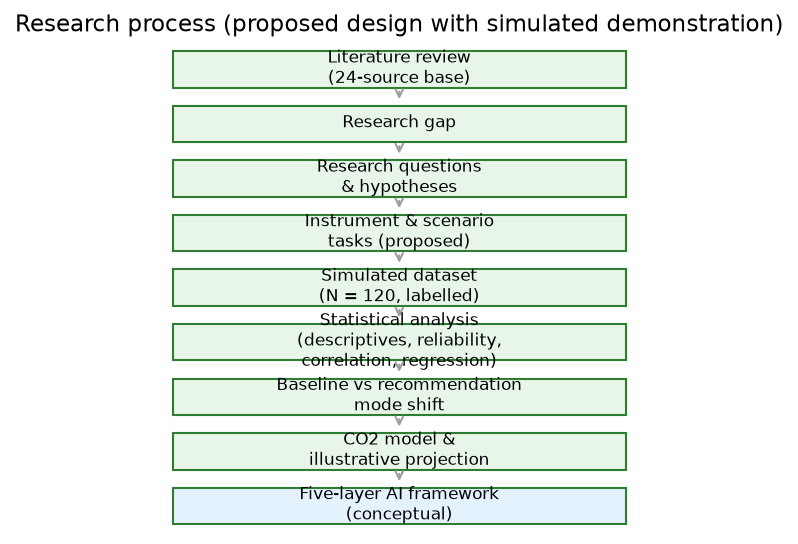
\includegraphics[width=0.72\textwidth]{fig_method_flow.png}
\caption{Research process: literature and gap lead to a proposed design and instrument, a labelled
simulated dataset, a full statistical demonstration, a scenario experiment and an emission projection,
and finally to the conceptual five-layer AI framework.}
\label{fig:flow}
\end{figure}

\section{Research Methodology}
\label{sec:method}

This study uses a \textbf{quantitative, cross-sectional, scenario-based research design with a
conceptual system-evaluation component}. The empirical version of the study would collect responses
from undergraduate students; in this paper, a simulated dataset is used to demonstrate the complete
analytical procedure. Throughout, the instrument, sampling and analysis are described as
\emph{proposed}, and every numerical result is described as a \emph{simulated demonstration}.

\subsection{Research Design}
The design is quantitative because it measures constructs numerically and tests hypotheses with
statistical procedures; cross-sectional because it observes respondents at a single point in time;
and scenario-based because mode choice is elicited through structured hypothetical trips rather than
observed travel. A within-subject baseline-versus-recommendation task adds a quasi-experimental
element, although it is hypothetical and therefore cannot establish causal effects. The conceptual
system-evaluation component maps each measured construct to a component of the proposed five-layer
assistant (Section~\ref{sec:framework}).

\subsection{Research Setting}
The proposed setting is the Gharuan campus of Chandigarh University, Punjab, India. The campus
attracts commuters from surrounding urban and semi-urban areas, which produces variation in commute
distance and available modes. The setting is a single institution, which limits generalisability
(Section~\ref{sec:limits}).

\subsection{Target Population}
The target population is undergraduate students who travel to campus at least three days per week.
Students who study fully online or who live on campus with no commuting trip are outside the
population of interest.

\subsection{Sampling Technique}
A convenience (non-probability) sample is proposed, recruited through departmental mailing lists and
class announcements. Convenience sampling is used because no sampling frame of commuting students is
available; the resulting selection bias is acknowledged as a limitation.

\subsection{Proposed Sample Size}
The target is $n \approx 150$ complete responses. This is adequate for descriptive analysis,
reliability estimation and the planned group comparisons, and is near the upper end of the common
10-observations-per-item guideline for factor analysis of a 40-item instrument; it is modest for the
logistic model and would constrain the number of predictors (Section~\ref{sec:limits}). No power
calculation is claimed, because no pilot variance estimate exists yet.

\subsection{Inclusion and Exclusion Criteria}
\textit{Inclusion:} age 18 or older; currently enrolled undergraduate; commutes to campus at least
three days per week; provides informed consent. \textit{Exclusion:} failed attention check;
completion time below one-third of the median (speeding); straight-lining across a Likert block.

\subsection{Research Instrument}
A self-administered online questionnaire with seven sections (A--G) is proposed. Section~A records
demographics and the commuting profile; Sections~B and~C measure sustainable-mobility awareness and
environmental concern; Section~D measures commuting decision factors; Section~E measures sustainable
travel intention; Section~F presents six scenario-based commute-choice tasks; and Section~G presents
personalised recommendation cards and measures assistant acceptance. The full instrument is in
Appendix~\ref{app:questionnaire}.

\subsection{Questionnaire Structure}
Table~\ref{tab:instr} summarises the structure. The instrument uses five-point Likert items and
single-choice scenario items. One unscored attention-check item is embedded in Section~B.

\begin{table}[H]
\centering
\small
\caption{Proposed questionnaire structure.}
\label{tab:instr}
\begin{tabular}{@{}llll@{}}
\toprule
\textbf{Section} & \textbf{Content} & \textbf{Items} & \textbf{Scale}\\
\midrule
A & Demographics and commuting profile & 7 & Categorical / count\\
B & Sustainable-mobility awareness & 9 (+1 attention) & 1--5 agreement\\
C & Environmental concern and attitudes & 7 & 1--5 agreement\\
D & Commuting decision factors & 12 & 1--5 agreement\\
E & Sustainable travel intention & 7 & 1--5 willingness\\
F & Scenario-based commute choice (Stage A) & 6 & Single choice\\
G1 & Recommendation response (Stage B/C) & 6 & Single choice\\
G2 & Assistant acceptance & 7 & 1--5 agreement\\
\bottomrule
\end{tabular}
\end{table}

\subsection{Scenario-Based Commute Choice Task}
Six scenarios (S1--S6) vary distance (3--15~km), context (weather, peak hour, first/last mile,
personal safety) and the option set (private car, city bus, metro/rail, bicycle, e-bike, carpool,
shared ride, and one multimodal metro$+$e-bike option). In Stage~A, respondents see travel time,
cost, comfort and convenience but \emph{not} estimated CO$_2$; they choose their preferred option. In
Stage~B they see a personalised recommendation card that displays travel time, cost, CO$_2$ impact,
convenience and an environmental-benefit statement. In Stage~C they choose again. Withholding CO$_2$
in Stage~A allows the effect of carbon information to be isolated. Scenario values are illustrative
design values, not measurements of real services in the Chandigarh region
(Appendix~\ref{app:scenarios}).

\subsection{Variables and Operational Definitions}
Variables, scales and coding are defined in Section~\ref{sec:operational} and the data dictionary in
Section~\ref{sec:datadict}.

\subsection{Scoring Procedure}
Scale scores are the arithmetic mean of their items (range 1--5), so that scores are comparable
across scales of different length. Mode choices are coded to categories; a \emph{sustainable}
(low-emission) choice is any option other than the solo private car. Emission variables use the model
in Section~\ref{sec:emission}. Full coding rules are in Appendix~\ref{app:coding}.

\subsection{Pilot Testing}
A pilot with approximately 15--20 students is proposed to assess wording clarity, completion time,
scenario realism and technical issues, and to obtain preliminary reliability estimates. Items with a
corrected item--total correlation below about $.30$, or scales with a preliminary alpha well below
$.70$, would be reviewed. Pilot data would be merged with main data only if the instrument is
unchanged.

\subsection{Validity}
Content validity is supported by grounding items in the reviewed literature
(Section~\ref{sec:lit}) and by review from the supervising faculty member and, ideally, two
additional subject experts. Face validity is assessed in the pilot. Construct validity would be
examined with exploratory factor analysis (if sample size permits), convergent patterns among related
scales and known-group differences (for example, private-vehicle users versus others). Criterion
validity against observed travel behaviour is not available in the present design.

\subsection{Reliability}
Internal consistency would be assessed with Cronbach's alpha for each multi-item scale (conventional
benchmark $\geq .70$, with lower values interpreted cautiously for short three-item scales) together
with corrected item--total correlations and alpha-if-item-deleted. The alpha values in
Section~\ref{sec:results} come from the simulated data and are demonstrations only.

\subsection{Data Collection Procedure}
Proposed procedure: eligible students receive an online link; consent is obtained before any question;
the six scenarios are presented in randomised order; Stage~B cards follow after all Stage~A choices
are completed; respondents receive an anonymous identifier. Typical completion time is expected to be
12--15 minutes (to be verified in the pilot).

\subsection{Data Cleaning}
Responses would be screened for completeness, failed attention checks, speeding and straight-lining.
Missing data below 5\% per scale would be handled by listwise deletion for composite scores.
Distributions would be inspected for outliers and data-entry errors. No cleaning has been performed
on genuine data because none exists.

\subsection{Statistical Analysis Plan}
All tests are two-tailed with $\alpha = .05$. Descriptive statistics (frequency, percentage, mean,
median, $SD$, minimum, maximum) address RQ1, RQ2 and RQ5. Cronbach's alpha assesses reliability.
Shapiro--Wilk tests and skewness/kurtosis guide the choice between parametric and non-parametric
procedures. Because Likert-derived scores are ordinal-like and frequently non-normal, Spearman
correlation is the default for association. Group comparisons use Welch's $t$-test when both groups
are approximately normal and the Mann--Whitney $U$ test otherwise; a Kruskal--Wallis test compares
intention across current-mode groups. A binary logistic regression addresses RQ3, and a conditional
(multinomial-logit-type) model examines the role of option attributes in Stage~A choices. Baseline and
post-recommendation choices are compared with the Wilcoxon signed-rank test on respondent-level
shares and McNemar's exact test on paired trip-level decisions (acknowledging clustering within
respondents); modelled CO$_2$ differences use a paired $t$-test or Wilcoxon test depending on
normality of the differences. Family-wise error across the seven hypothesis tests is described with
Holm-adjusted $p$-values. Effect sizes accompany tests.

\begin{table}[H]
\centering
\small
\caption{Research question--variable--analysis mapping.}
\label{tab:rqmap}
\begin{tabular}{@{}p{1.0cm}p{4.6cm}p{4.0cm}p{4.4cm}@{}}
\toprule
\textbf{RQ} & \textbf{Variables} & \textbf{Analysis} & \textbf{Decision rule}\\
\midrule
RQ1 & \code{awareness\_score}; \code{concern\_score} & Descriptives; Wilcoxon vs midpoint 3 & $p < .05$\\
RQ2 & \code{intention\_score}; \code{private\_vehicle\_user} & Descriptives; Welch $t$ / Mann--Whitney $U$ & $p < .05$\\
RQ3 & \code{low\_emission\_majority}; six predictors & Binary logistic regression & LR test $p < .05$; Wald tests\\
RQ4 & awareness, concern, intention, \code{shift\_count} & Spearman $\rho$ & $p < .05$\\
RQ5 & \code{acceptance\_score}; \code{convenience\_score} & Descriptives; Spearman $\rho$ & $p < .05$\\
RQ6 & \code{car\_share}, \code{estimated\_co2\_saved} & Wilcoxon; McNemar; paired $t$ / Wilcoxon & $p < .05$\\
\bottomrule
\end{tabular}
\end{table}

\subsection{Ethical Considerations}
Participation would be voluntary, with informed consent obtained at the start and the right to
withdraw. Responses are anonymous and used only for academic purposes; no passwords, financial
details or directly identifying information are collected. Data would be stored securely.
Institutional or supervisor approval will be obtained where required before any genuine data
collection. No human participants were involved in the present paper, because all numerical data are
simulated.

\section{Research Instrument (Questionnaire)}
This section summarises the proposed questionnaire; the full participant-facing text, with response
anchors, is in Appendix~\ref{app:questionnaire} and the scenario cards in
Appendix~\ref{app:scenarios}. The instrument is proposed, has not been piloted and has not been
administered to any participant.

\subsection{Section A --- Demographic and Commuting Profile}
Age (years); gender; year of study; programme; one-way commute-distance category ($<2$~km, 2--5~km,
5--10~km, $>10$~km); main current commuting mode (private car, two-wheeler, bus [public or
university], walking/cycling, carpool/shared ride); and commuting days per week.

\subsection{Section B --- Sustainable Mobility Awareness}
Nine agreement items ($1 =$ strongly disagree to $5 =$ strongly agree) plus one unscored
attention-check item. Items address knowledge of low-emission options, awareness of the contribution
of private cars, active and shared modes, the grid-dependence of EV benefits, digital tools and the
ability to compare CO$_2$ impact (items aw1--aw9, Appendix~\ref{app:questionnaire}).

\subsection{Section C --- Environmental Concern and Attitudes}
Seven agreement items (ec1--ec7) covering concern about air pollution and climate change, personal
responsibility, belief in the effect of individual choices, institutional encouragement and
willingness to accept a slightly longer trip for lower emissions.

\subsection{Section D --- Commuting Decision Factors}
Twelve agreement items: three each for cost sensitivity (cost1--3), time sensitivity (time1--3) and
perceived convenience (conv1--3), and one single item each for comfort, safety and accessibility.

\subsection{Section E --- Sustainable Travel Intention}
Seven willingness items ($1 =$ very unwilling to $5 =$ very willing) for the next semester: walking,
cycling, public transport, carpooling, shared mobility, e-bike/e-scooter and electric vehicles.

\subsection{Section F --- Scenario-Based Commute Choice (Stage A)}
Six scenarios (S1--S6) as summarised in Table~\ref{tab:scenarios}. In each, the respondent selects the
option they would choose for the trip described.

\begin{table}[H]
\centering
\small
\caption{Overview of scenario-based commute-choice tasks (design values; full option cards in
Appendix~\ref{app:scenarios}).}
\label{tab:scenarios}
\begin{tabular}{@{}p{0.8cm}p{6.0cm}p{1.4cm}p{5.6cm}@{}}
\toprule
\textbf{ID} & \textbf{Context} & \textbf{Distance} & \textbf{Options presented}\\
\midrule
S1 & Short campus-area trip, fair weather, off-peak & 3~km & Private car, City bus, Bicycle, E-bike, Shared ride\\
S2 & Peak-hour trip, congested corridor & 6~km & Private car, City bus, Bicycle, Carpool, E-bike\\
S3 & Hot, humid day, medium distance & 8~km & Private car, City bus, Metro/rail, Carpool, Shared ride\\
S4 & Rainy day, longer distance & 12~km & Private car, City bus, Metro/rail, Carpool, Shared ride\\
S5 & Long trip with first/last-mile leg (multimodal) & 15~km & Private car, Metro $+$ e-bike, City bus, Carpool, Shared ride\\
S6 & Evening return trip, personal-safety concern & 5~km & Private car, City bus, Carpool, Shared ride, E-bike\\
\bottomrule
\end{tabular}
\end{table}

\subsection{Section G --- Smart Commute Assistant Acceptance}
Part~G1 shows, for each scenario, a personalised recommendation card (Stage~B) and records the
post-recommendation choice (Stage~C). Part~G2 contains seven agreement items on perceived usefulness,
trust, recommendation acceptance, willingness to follow suggestions, perceived environmental value,
intention to continue use and intention to check carbon feedback. The first six form the acceptance
scale (the item on continued use is shared with the user-engagement index).

\section{Operational Definitions of Variables}
\label{sec:operational}

Table~\ref{tab:opdef} maps each construct to its variable, measurement, scale, basis in the
literature and the analysis in which it is used. Composite scores are the arithmetic mean of their
items and therefore range from 1 to 5.

\begin{table}[H]
\centering
\small
\caption{Constructs, variables, operational definitions and analysis.}
\label{tab:opdef}
\resizebox{\textwidth}{!}{%
\begin{tabular}{@{}p{2.3cm}p{2.6cm}p{3.3cm}p{1.4cm}p{2.3cm}p{2.1cm}@{}}
\toprule
\textbf{Construct} & \textbf{Variable} & \textbf{Measurement} & \textbf{Scale} & \textbf{Basis} & \textbf{Analysis}\\
\midrule
Environmental awareness & \code{awareness\_score} & Mean of aw1--aw9 & 1--5 & \citet{eslami2025,bamberg2007} & RQ1, RQ3, RQ4; $t$-test\\
Environmental concern & \code{concern\_score} & Mean of ec1--ec7 & 1--5 & \citet{bamberg2007} & RQ1, RQ3, RQ4; Spearman\\
Sustainable travel intention & \code{intention\_score} & Mean of int1--int7 & 1--5 & \citet{bamberg2007,lattman2024} & RQ2, RQ4; $t$-test, Kruskal--Wallis\\
Cost sensitivity & \code{cost\_sensitivity} & Mean of cost1--3 & 1--5 & \citet{wu2025} & RQ3; logistic regression\\
Time sensitivity & \code{time\_sensitivity} & Mean of time1--3 & 1--5 & \citet{wu2025} & RQ3; logistic regression\\
Perceived convenience & \code{convenience\_score} & Mean of conv1--3 & 1--5 & \citet{smith2023} & RQ3, RQ5; Spearman\\
Comfort, safety, accessibility & \code{comfort}, \code{safety}, \code{access} & Single items & 1--5 & \citet{cui2024,marzolla2025} & Descriptives\\
Recommendation acceptance & \code{acceptance\_score} & Mean of acc1--acc6 & 1--5 & \citet{eslami2025,niazi2024} & RQ5; Spearman\\
User engagement & \code{engagement} & Mean of acc6, acc7 & 1--5 & \citet{niazi2024,sunio2018} & Descriptives\\
Sustainable mode choice & \code{low\_emission\_majority} & 1 if $\geq 4$ of 6 Stage~A choices are non-car & 0/1 & \citet{comi2024} & RQ3; logistic regression\\
Mode shift & \code{shift\_count}, \code{mode\_shift\_indicator} & Number of car$\rightarrow$non-car changes & Count / 0/1 & \citet{eslami2025} & RQ4; Spearman\\
Estimated CO$_2$ savings & \code{estimated\_co2\_saved} & Baseline $-$ recommended emission (g) & Continuous & \citet{ndhlovu2025} & RQ6; paired $t$/Wilcoxon\\
\bottomrule
\end{tabular}}
\end{table}

\section{Data Dictionary}
\label{sec:datadict}

Table~\ref{tab:datadict} lists the respondent-level variables. Likert items are integers from 1 to 5
with no reverse-keyed items. Composite scores are arithmetic means. Scenario variables store a
single-letter mode code: C private car, B city bus, M metro/rail, Y bicycle, E e-bike, P carpool,
S shared ride, X metro$+$e-bike (Appendix~\ref{app:coding}).

\footnotesize
\begin{longtable}{@{}p{3.5cm}p{1.9cm}p{8.2cm}@{}}
\caption{Respondent-level data dictionary (simulated dataset structure).}
\label{tab:datadict}\\
\toprule
\textbf{Variable} & \textbf{Type / range} & \textbf{Description}\\
\midrule
\endfirsthead
\toprule
\textbf{Variable} & \textbf{Type / range} & \textbf{Description}\\
\midrule
\endhead
\bottomrule
\endlastfoot
\code{respondent\_id} & String & Anonymous identifier (R001--R120)\\
\code{age} & Integer 18--23 & Age in years\\
\code{gender} & Categorical & Male / Female / Other-prefer not to say\\
\code{year\_of\_study} & Integer 1--4 & Current year of undergraduate study\\
\code{programme} & Categorical & CSE / Other engineering / Management-Commerce / Sciences-Other\\
\code{commute\_distance\_cat} & Categorical & $<$2 / 2--5 / 5--10 / $>$10 km (one way)\\
\code{current\_mode} & Categorical & Private car / Two-wheeler / Bus / Walking-Cycling / Carpool-Shared\\
\code{commute\_days} & Integer 3--6 & Days per week travelling to campus\\
\code{aw1}--\code{aw9} & Likert 1--5 & Sustainable-mobility awareness items\\
\code{ec1}--\code{ec7} & Likert 1--5 & Environmental-concern items\\
\code{cost1}--\code{cost3} & Likert 1--5 & Cost-sensitivity items\\
\code{time1}--\code{time3} & Likert 1--5 & Time-sensitivity items\\
\code{conv1}--\code{conv3} & Likert 1--5 & Convenience items\\
\code{comfort}, \code{safety}, \code{access} & Likert 1--5 & Single-item comfort, safety and accessibility\\
\code{int1}--\code{int7} & Likert 1--5 & Sustainable travel intention items (walk, cycle, PT, carpool, shared, e-bike, EV)\\
\code{acc1}--\code{acc7} & Likert 1--5 & Assistant acceptance and engagement items\\
\code{attention\_check} & Integer 1--5 & Unscored quality-control item (correct $=4$)\\
\code{stageA\_S1}--\code{stageA\_S6} & Mode code & Baseline (pre-recommendation) choice per scenario\\
\code{rec\_S1}--\code{rec\_S6} & Mode code & Personalised recommended mode per scenario\\
\code{stageC\_S1}--\code{stageC\_S6} & Mode code & Post-recommendation choice per scenario\\
\code{emission\_A\_S1}--\code{emission\_A\_S6} & Numeric (g) & Modelled CO$_2$ for the baseline choice\\
\code{emission\_C\_S1}--\code{emission\_C\_S6} & Numeric (g) & Modelled CO$_2$ for the post-recommendation choice\\
\code{awareness\_score} & Numeric 1--5 & Mean of aw1--aw9\\
\code{concern\_score} & Numeric 1--5 & Mean of ec1--ec7\\
\code{cost\_sensitivity} & Numeric 1--5 & Mean of cost1--cost3\\
\code{time\_sensitivity} & Numeric 1--5 & Mean of time1--time3\\
\code{convenience\_score} & Numeric 1--5 & Mean of conv1--conv3\\
\code{intention\_score} & Numeric 1--5 & Mean of int1--int7\\
\code{acceptance\_score} & Numeric 1--5 & Mean of acc1--acc6\\
\code{engagement} & Numeric 1--5 & Mean of acc6 and acc7\\
\code{total\_awareness\_score} & Numeric 9--45 & Sum of aw1--aw9 (for reporting)\\
\code{total\_intention\_score} & Numeric 7--35 & Sum of int1--int7\\
\code{total\_acceptance\_score} & Numeric 6--30 & Sum of acc1--acc6\\
\code{private\_vehicle\_user} & 0/1 & 1 if current mode is private car or two-wheeler\\
\code{low\_emission\_majority} & 0/1 & 1 if $\geq 4$ of 6 Stage~A choices are non-car\\
\code{car\_share\_A}, \code{car\_share\_C} & Numeric 0--1 & Proportion of the six choices that are car\\
\code{sust\_share\_A}, \code{sust\_share\_C} & Numeric 0--1 & Proportion of the six choices that are non-car\\
\code{baseline\_emission} & Numeric (g) & Mean modelled CO$_2$ across the six baseline choices\\
\code{recommended\_emission} & Numeric (g) & Mean modelled CO$_2$ across the six post-recommendation choices\\
\code{estimated\_co2\_saved} & Numeric (g) & \code{baseline\_emission} $-$ \code{recommended\_emission}\\
\code{shift\_count} & Integer 0--6 & Number of scenarios changing from car to non-car\\
\code{mode\_shift\_indicator} & 0/1 & 1 if \code{shift\_count} $\geq 1$\\
\code{selected\_mode} & Mode code & Representative selected mode (Stage~C, S1)\\
\end{longtable}

\section{Emission Model}
\label{sec:emission}

Emissions are estimated with a transparent distance--factor model. For a trip made by a single mode
$m$,
\begin{equation}
E_m = d \times EF_m,
\label{eq:single}
\end{equation}
where $E_m$ is the estimated emissions for mode $m$ (grams of CO$_2$), $d$ is the passenger travel
distance (kilometres) and $EF_m$ is the emission factor for mode $m$ (grams of CO$_2$ per
passenger-kilometre). For a route comprising several legs,
\begin{equation}
E_{\text{total}} = \sum_{i} \left( d_i \times EF_i \right).
\label{eq:multi}
\end{equation}
Relative to a private-car baseline, the modelled saving is
\begin{equation}
\text{CO}_2\text{ saved} = E_{\text{car}} - E_{\text{selected}}.
\label{eq:saved}
\end{equation}
The multimodal metro$+$e-bike option (code X) is evaluated with Equation~\ref{eq:multi} as a
distance-weighted combination of its legs.

The emission factors used in the simulated demonstration are listed in Table~\ref{tab:ef}. They are
\textbf{illustrative model inputs only}. Real implementation would require region-specific, validated
emission factors that reflect local fleet composition, occupancy, fuel type and grid mix; the
electric-mode factor in particular depends on how electricity is generated \citep{ndhlovu2025}.
Bus, carpool and shared-ride factors represent emissions allocated per passenger under assumed
occupancies. No universal fixed emission value is claimed.

\begin{table}[H]
\centering
\small
\caption{Illustrative emission factors used in the simulated demonstration (g CO$_2$ per
passenger-km). These are model inputs, not measured values for the Chandigarh region.}
\label{tab:ef}
\begin{tabular}{@{}llcc@{}}
\toprule
\textbf{Code} & \textbf{Mode} & \textbf{$EF_m$ (g/pkm)} & \textbf{Note}\\
\midrule
C & Private car (solo) & 170 & Reference baseline\\
B & City bus & 70 & Allocated per passenger, assumed occupancy\\
M & Metro / rail & 30 & Allocated per passenger\\
Y & Bicycle & 0 & No tailpipe emissions modelled\\
E & E-bike / e-scooter & 20 & Grid-dependent in reality\\
P & Carpool & 57 & Car factor $\div$ assumed occupancy 3\\
S & Shared ride & 60 & Car factor $\div$ assumed occupancy $\approx$ 2.8\\
X & Metro $+$ e-bike & 42 & Distance-weighted multimodal combination\\
\bottomrule
\end{tabular}
\end{table}

Applying Equation~\ref{eq:single} to each scenario's distance gives the all-car reference emissions
shown in Table~\ref{tab:co2} (Section~\ref{sec:results}); for example, the 8~km scenario (S3) has an
all-car reference of $8 \times 170 = 1360$~g.

\section{Simulated Demonstration Dataset}
\label{sec:dataset}

\textbf{Purpose and status.} A synthetic dataset of $N = 120$ respondents was generated with a
computer program (Python; NumPy; fixed random seed \code{20251006}) to demonstrate the analysis
procedure. It is \emph{not} real data. The respondents are fictional; they are not Chandigarh
University students and no real person provided any value. The generation script and the resulting
dataset accompany this paper so that the demonstration is fully reproducible.

\textbf{Generation procedure.} (1)~Demographics and commute-distance categories were drawn from
assumed distributions, and the current mode was drawn conditional on distance. (2)~Latent traits
(awareness, concern, convenience, cost sensitivity, time sensitivity, intention, acceptance and
engagement) were drawn from correlated normal distributions with modest offsets for private-vehicle
users. (3)~Likert items were generated from latent traits plus independent noise, rounded and clipped
to 1--5, so that scales are imperfectly reliable and values are not perfectly correlated.
(4)~Stage~A scenario choices were generated from a random-utility (multinomial-logit-type) model with
terms for travel time, cost, comfort, convenience, emissions and a current-mode inertia term.
(5)~Personalised recommendations were generated by ranking options with respondent-specific weights on
time, cost and CO$_2$. (6)~Stage~C choices followed the recommendation with a probability that
increased with the acceptance score and, weakly, with environmental concern; otherwise the Stage~A
choice was retained.

\textbf{Consequences for interpretation.} Associations such as awareness--intention and
convenience--acceptance were deliberately built into the generator, so detecting them demonstrates
that the procedure works and is not evidence about real commuters. The weak concern effect on
following recommendations was built in at a small size, so a non-significant result illustrates
limited power for small effects. Where the generator contains no effect, test results show how null
results would be reported. The recommendation rule never recommends an option worse than all
alternatives on its own weighted criteria, and the generator allows Stage~C to differ from Stage~A
only through following a recommendation, so patterns such as a decline in car share are partly built
in. Agreement with any published study would likewise be by construction and carries no evidential
weight.

\textbf{Plausibility checks.} Scale means lie between 3.46 and 3.65 (not at ceiling), scale
reliabilities range from the questionable to the good range, correlations are moderate rather than
near-perfect, and baseline private-car share ($35.0\%$ of decisions) is plausible for a scenario set
that includes short and long trips. These checks establish internal plausibility only. The complete
respondent-level dataset is provided as an accompanying data file (Appendix~\ref{app:dataset}); a
representative extract is shown in Table~\ref{tab:extract}.

\section{Results and Data Analysis}
\label{sec:results}

\begin{center}
\fbox{\parbox{0.93\textwidth}{\small
\textbf{The numerical results in this section are generated from a simulated demonstration dataset
and are intended solely to illustrate the proposed analysis procedure. They do not represent actual
students or actual system deployment outcomes.}}}
\end{center}

All analyses use the $N = 120$ simulated respondents of Appendix~\ref{app:dataset} and were computed
in Python (pandas, SciPy, statsmodels). Tests are two-tailed with $\alpha = .05$. Because the data
were generated with built-in structure (Section~\ref{sec:dataset}), significance here demonstrates
that the analytical procedure functions and does not support any claim about real commuters or any
real system.

\subsection{Simulated Participant Profile}
The simulated respondents were aged 18--23 years ($M = 19.86$, $SD = 1.29$). $58.3\%$ were male,
$38.3\%$ female and $3.3\%$ other/prefer not to say. $42.5\%$ mainly used a private car or
two-wheeler. Table~\ref{tab:profile} and Figure~\ref{fig:profile} show the profile.

\begin{table}[H]
\centering
\small
\caption{Simulated participant profile (simulated demonstration data, $N = 120$).}
\label{tab:profile}
\begin{tabular}{@{}llrr@{}}
\toprule
\textbf{Variable} & \textbf{Category} & \textbf{$n$} & \textbf{\%}\\
\midrule
\multirow{3}{*}{Gender} & Male & 70 & 58.3\%\\
 & Female & 46 & 38.3\%\\
 & Other/Prefer not to say & 4 & 3.3\%\\
\midrule
\multirow{4}{*}{Year of study} & 1 & 34 & 28.3\%\\
 & 2 & 45 & 37.5\%\\
 & 3 & 31 & 25.8\%\\
 & 4 & 10 & 8.3\%\\
\midrule
\multirow{4}{*}{Programme} & CSE & 47 & 39.2\%\\
 & Other engineering & 38 & 31.7\%\\
 & Management/Commerce & 27 & 22.5\%\\
 & Sciences/Other & 8 & 6.7\%\\
\midrule
\multirow{4}{*}{Commute distance (one-way)} & $<$2~km & 26 & 21.7\%\\
 & 2--5~km & 33 & 27.5\%\\
 & 5--10~km & 33 & 27.5\%\\
 & $>$10~km & 28 & 23.3\%\\
\midrule
\multirow{5}{*}{Current mode} & Private car & 22 & 18.3\%\\
 & Two-wheeler & 29 & 24.2\%\\
 & Bus (public/university) & 24 & 20.0\%\\
 & Walking/Cycling & 26 & 21.7\%\\
 & Carpool/Shared ride & 19 & 15.8\%\\
\midrule
\multirow{4}{*}{Commuting days per week} & 3 & 10 & 8.3\%\\
 & 4 & 17 & 14.2\%\\
 & 5 & 49 & 40.8\%\\
 & 6 & 44 & 36.7\%\\
\bottomrule
\end{tabular}
\end{table}

\begin{figure}[H]
\centering
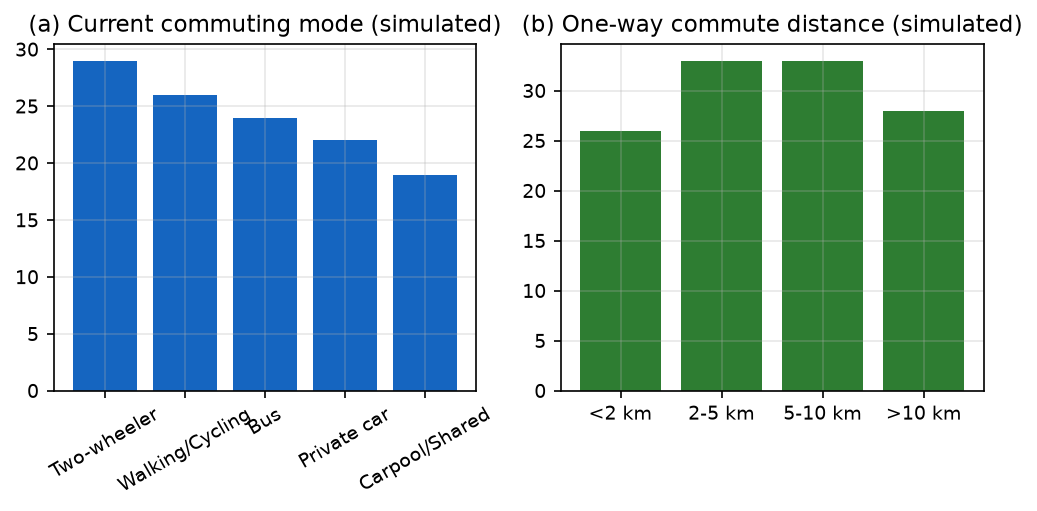
\includegraphics[width=0.9\textwidth]{fig_profile.png}
\caption{Respondent and commuting profile of the simulated demonstration dataset ($N = 120$):
(a) current commuting mode; (b) one-way commute distance.}
\label{fig:profile}
\end{figure}

\subsection{Sustainable Mobility Awareness}
Mean awareness was $3.52$ ($SD = 0.76$; median $= 3.56$; range $1.67$--$4.89$), above the scale
midpoint of 3 (one-sample Wilcoxon signed-rank, $p < .001$). $30.0\%$ of simulated respondents scored
$4.00$ or higher. Table~\ref{tab:awareness} gives item-level results and Figure~\ref{fig:awareness}
the distribution. RQ1 is therefore illustrated as moderate-to-high simulated awareness; this reflects
generator settings and is not an estimate for real students.

\begin{table}[H]
\centering
\small
\caption{Awareness items (simulated demonstration data, $N = 120$).}
\label{tab:awareness}
\begin{tabular}{@{}lrrr@{}}
\toprule
\textbf{Item} & \textbf{$M$} & \textbf{$SD$} & \textbf{Agree (4--5)}\\
\midrule
Knows which options emit less CO$_2$ than a car & 3.51 & 1.14 & 51.7\%\\
Understands car commuting contributes to emissions & 3.61 & 1.25 & 54.2\%\\
Aware public transport can emit less per passenger-km & 3.49 & 1.05 & 50.0\%\\
Knows walking/cycling have almost no tailpipe emissions & 3.48 & 1.19 & 51.7\%\\
Aware carpooling reduces vehicles on the road & 3.52 & 1.10 & 50.0\%\\
Aware shared e-bikes/e-scooters can replace short car trips & 3.55 & 1.05 & 52.5\%\\
Understands EV benefit depends on electricity source & 3.51 & 1.04 & 52.5\%\\
Knows apps showing multimodal routes/emissions & 3.58 & 1.15 & 56.7\%\\
Can judge which option has lower CO$_2$ & 3.43 & 1.14 & 57.5\%\\
\bottomrule
\end{tabular}
\end{table}

\begin{figure}[H]
\centering
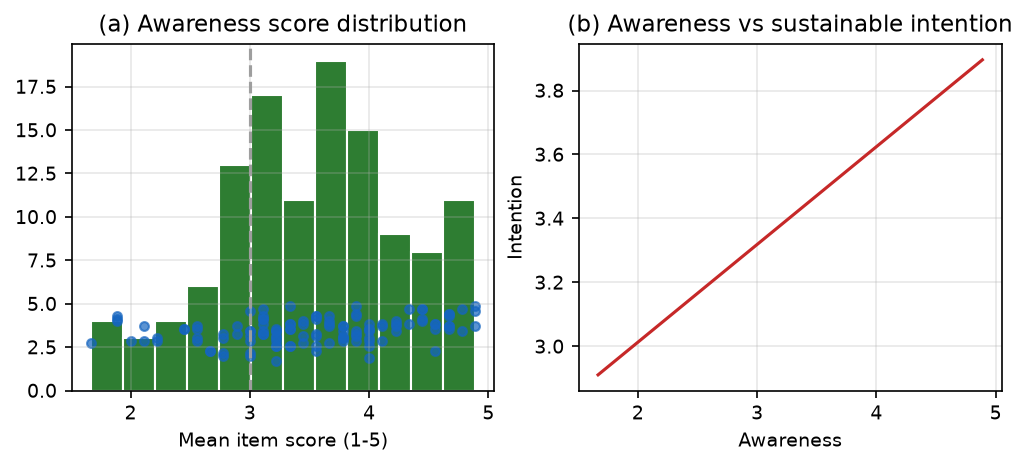
\includegraphics[width=0.9\textwidth]{fig_awareness.png}
\caption{(a) Distribution of environmental awareness scores in the simulated dataset
($N = 120$); (b) awareness versus sustainable travel intention, with a linear trend line for
illustration.}
\label{fig:awareness}
\end{figure}

\subsection{Environmental Concern and Attitudes}
Mean environmental concern was $3.65$ ($SD = 0.72$; median $= 3.71$). Agreement was highest for
``feels personal responsibility for travel emissions'' and lowest for ``concerned about transport
emissions and climate'' (Table~\ref{tab:concern}).

\begin{table}[H]
\centering
\small
\caption{Environmental-concern items (simulated demonstration data, $N = 120$).}
\label{tab:concern}
\begin{tabular}{@{}lrrr@{}}
\toprule
\textbf{Item} & \textbf{$M$} & \textbf{$SD$} & \textbf{Agree (4--5)}\\
\midrule
Concerned about road-traffic air pollution & 3.64 & 1.09 & 60.0\%\\
Concerned about transport emissions and climate & 3.52 & 1.20 & 55.0\%\\
Feels personal responsibility for travel emissions & 3.76 & 1.08 & 60.8\%\\
Uncomfortable choosing high-emission option when cleaner exists & 3.69 & 1.04 & 54.2\%\\
Believes individual choices make a difference & 3.65 & 1.03 & 55.8\%\\
Universities should encourage low-emission commuting & 3.66 & 1.03 & 55.8\%\\
Emission reduction important even if slightly slower & 3.62 & 1.05 & 57.5\%\\
\bottomrule
\end{tabular}
\end{table}

\subsection{Commuting Behaviour and Decision Factors}
In the simulated data, convenience ($M = 3.55$, $SD = 0.76$), time sensitivity ($M = 3.53$,
$SD = 0.80$) and cost sensitivity ($M = 3.46$, $SD = 0.86$) were the stated decision factors, with
single-item comfort, safety and accessibility ratings shown in Table~\ref{tab:factors}. Current-mode
shares are in Figure~\ref{fig:profile}. Full descriptive statistics for all composite scores,
including median, range, skewness, excess kurtosis and the Shapiro--Wilk test, are given in
Table~\ref{tab:desc}.

\begin{table}[H]
\centering
\small
\caption{Commuting decision factors (simulated demonstration data, $N = 120$).}
\label{tab:factors}
\begin{tabular}{@{}lrrr@{}}
\toprule
\textbf{Factor} & \textbf{$M$} & \textbf{$SD$} & \textbf{Median}\\
\midrule
Cost sensitivity (3 items) & 3.46 & 0.86 & 3.67\\
Time sensitivity (3 items) & 3.53 & 0.80 & 3.50\\
Perceived convenience (3 items) & 3.55 & 0.76 & 3.67\\
Comfort (1 item) & 3.70 & 1.00 & 4.00\\
Safety (1 item) & 3.62 & 1.05 & 4.00\\
Accessibility (1 item) & 3.61 & 1.04 & 4.00\\
\bottomrule
\end{tabular}
\end{table}

\begin{table}[H]
\centering
\small
\caption{Descriptive statistics and distribution assessment of composite scores (simulated
demonstration data, $N = 120$).}
\label{tab:desc}
\begin{tabular}{@{}lrrrrrrrr@{}}
\toprule
\textbf{Score} & \textbf{$M$} & \textbf{$SD$} & \textbf{Mdn} & \textbf{Min} & \textbf{Max} & \textbf{Skew} & \textbf{Kurt.} & \textbf{SW $p$}\\
\midrule
Awareness (aw) & 3.52 & 0.76 & 3.56 & 1.67 & 4.89 & $-0.22$ & $-0.43$ & .078\\
Concern (ec) & 3.65 & 0.72 & 3.71 & 1.57 & 5.00 & $-0.41$ & $-0.26$ & .034\\
Cost sensitivity & 3.46 & 0.86 & 3.67 & 1.00 & 5.00 & $-0.29$ & $-0.32$ & .013\\
Time sensitivity & 3.53 & 0.80 & 3.50 & 1.33 & 5.00 & $-0.33$ & $-0.46$ & .002\\
Convenience & 3.55 & 0.76 & 3.67 & 1.33 & 5.00 & $-0.12$ & $-0.50$ & .003\\
Intention & 3.48 & 0.72 & 3.57 & 1.71 & 4.86 & $-0.18$ & $-0.41$ & .184\\
Acceptance & 3.56 & 0.72 & 3.67 & 1.83 & 5.00 & $-0.33$ & $-0.42$ & .039\\
Engagement & 3.54 & 0.88 & 3.50 & 1.50 & 5.00 & $-0.32$ & $-0.44$ & $<.001$\\
\bottomrule
\end{tabular}
\end{table}

\subsection{Sustainable Travel Intention}
Mean sustainable travel intention was $3.48$ ($SD = 0.72$; median $= 3.57$), above the midpoint
(Wilcoxon $p < .001$). Willingness was highest for walking and lowest for carpooling
(Table~\ref{tab:intention}).

\begin{table}[H]
\centering
\small
\caption{Mode-specific sustainable travel intention (simulated demonstration data, $N = 120$).}
\label{tab:intention}
\begin{tabular}{@{}lrrr@{}}
\toprule
\textbf{Mode} & \textbf{$M$} & \textbf{$SD$} & \textbf{Willing (4--5)}\\
\midrule
Walking & 3.57 & 1.06 & 51.7\%\\
Cycling & 3.46 & 1.11 & 55.0\%\\
Public transport & 3.50 & 1.13 & 53.3\%\\
Carpooling & 3.41 & 1.05 & 47.5\%\\
Shared mobility & 3.48 & 1.07 & 55.0\%\\
E-bike/e-scooter & 3.42 & 1.07 & 50.0\%\\
Electric vehicle & 3.51 & 1.17 & 58.3\%\\
\bottomrule
\end{tabular}
\end{table}

\subsection{Reliability Analysis}
Cronbach's alpha was computed on the simulated items for each multi-item scale
(Table~\ref{tab:reliability}). Awareness ($\alpha = .85$), concern ($\alpha = .79$), intention
($\alpha = .78$) and acceptance ($\alpha = .74$) reached the conventional benchmark of $.70$; the
three-item cost ($\alpha = .68$), time ($\alpha = .58$) and convenience ($\alpha = .54$) scales fell
below it. These values are demonstrations calculated from simulated data; they do not establish the
reliability of the instrument with real respondents, and the short three-item scales would require
review before the main survey.

\begin{table}[H]
\centering
\small
\caption{Reliability of multi-item scales (simulated demonstration data, $N = 120$).}
\label{tab:reliability}
\begin{tabular}{@{}lcc@{}}
\toprule
\textbf{Scale} & \textbf{Items} & \textbf{Cronbach's $\alpha$}\\
\midrule
Awareness & 9 & .85\\
Environmental concern & 7 & .79\\
Sustainable travel intention & 7 & .78\\
Assistant acceptance & 6 & .74\\
Cost sensitivity & 3 & .68\\
Time sensitivity & 3 & .58\\
Convenience & 3 & .54\\
\bottomrule
\end{tabular}
\end{table}

\subsection{Correlation Analysis}
Awareness and intention were positively correlated (Spearman $\rho = .34$, $p < .001$; H1).
Convenience and assistant acceptance were weakly-to-moderately positively correlated ($\rho = .21$,
$p = .023$; H3). Environmental concern and the number of car-to-sustainable shifts after
recommendation were not significantly correlated ($\rho = .03$, $p = .785$; H2). Correlation does not
imply causation; relationships here were partly built into the generator. Table~\ref{tab:corr} shows
the full matrix and Figure~\ref{fig:awareness}(b) the awareness--intention relationship.

\begin{table}[H]
\centering
\small
\caption{Spearman correlation matrix (simulated demonstration data, $N = 120$).
$^{*}p<.05$, $^{**}p<.01$, $^{***}p<.001$.}
\label{tab:corr}
\begin{tabular}{@{}lrrrrrrr@{}}
\toprule
 & Aware. & Concern & Intent. & Conv. & Cost & Time & Accept.\\
\midrule
Awareness & --- & $.23^{*}$ & $.34^{***}$ & $-.15$ & $-.14$ & $.20^{*}$ & $.14$\\
Concern & $.23^{*}$ & --- & $.22^{*}$ & $-.20^{*}$ & $-.14$ & $-.10$ & $.16$\\
Intention & $.34^{***}$ & $.22^{*}$ & --- & $-.15$ & $-.10$ & $.03$ & $.12$\\
Convenience & $-.15$ & $-.20^{*}$ & $-.15$ & --- & $-.05$ & $-.02$ & $.21^{*}$\\
Cost sens. & $-.14$ & $-.14$ & $-.10$ & $-.05$ & --- & $.03$ & $-.16$\\
Time sens. & $.20^{*}$ & $-.10$ & $.03$ & $-.02$ & $.03$ & --- & $.10$\\
Acceptance & $.14$ & $.16$ & $.12$ & $.21^{*}$ & $-.16$ & $.10$ & ---\\
\bottomrule
\end{tabular}
\end{table}

\subsection{Group Comparisons}
Three exploratory grouping comparisons were run. The private-vehicle comparison corresponds to H4.
For each outcome, the test was chosen after Shapiro--Wilk checks of both groups
(Table~\ref{tab:groups}). Private-vehicle users scored $3.27$ versus $3.63$ for others on sustainable
intention ($t(103.9) = -2.83$, $p = .006$, $d = -0.53$), so H4 was supported in this simulated
sample. High-awareness respondents reported higher intention: the median split gave $3.66$ versus
$3.28$ ($t(116.9) = 3.00$, $p = .003$, $d = 0.55$), which is expected from the correlation in
Section~\ref{sec:results} and from how the data were generated. Distance-group
differences were small and non-significant. A Kruskal--Wallis test across the five current-mode
groups was not significant ($H(4) = 8.36$, $p = .079$).

\begin{table}[H]
\centering
\small
\caption{Group comparisons (simulated demonstration data, $N = 120$). Cells show $M$ ($SD$); share
variables are on a 0--1 scale and CO$_2$ saved is g per trip.}
\label{tab:groups}
\resizebox{\textwidth}{!}{%
\begin{tabular}{@{}p{3.4cm}p{2.4cm}rrll@{}}
\toprule
\textbf{Comparison} & \textbf{Outcome} & \textbf{Group 1} & \textbf{Group 2} & \textbf{Test} & \textbf{Effect}\\
\midrule
Private vehicle ($n=51$) vs other ($n=69$) & Sustainable intention & 3.27 (0.72) & 3.63 (0.68) & $t(103.9)=-2.83$, $p=.006$ & $d=-0.53$\\
 & Environmental awareness & 3.46 (0.71) & 3.56 (0.79) & $t(113.7)=-0.73$, $p=.468$ & $d=-0.13$\\
 & Assistant acceptance & 3.54 (0.73) & 3.57 (0.71) & $t(106.4)=-0.25$, $p=.803$ & $d=-0.05$\\
\midrule
Short $<$5~km ($n=59$) vs long $\geq$5~km ($n=61$) & Sustainable intention & 3.51 (0.76) & 3.45 (0.68) & $t(115.5)=0.46$, $p=.643$ & $d=0.09$\\
 & Car share at baseline & 0.34 (0.27) & 0.36 (0.23) & $U=1666.0$, $p=.476$ & $r_{rb}=0.07$\\
 & CO$_2$ saved/trip (g) & 125.7 (168.9) & 142.3 (191.3) & $U=1684.5$, $p=.538$ & $r_{rb}=0.06$\\
\midrule
High ($n=62$) vs low awareness ($n=58$) & Sustainable intention & 3.66 (0.68) & 3.28 (0.71) & $t(116.9)=3.00$, $p=.003$ & $d=0.55$\\
 & Assistant acceptance & 3.70 (0.69) & 3.41 (0.71) & $t(116.9)=2.22$, $p=.028$ & $d=0.41$\\
 & Baseline sustainable share & 0.70 (0.23) & 0.60 (0.27) & $U=2159.5$, $p=.053$ & $r_{rb}=0.20$\\
\bottomrule
\end{tabular}}
\end{table}

\subsection{Regression Analysis}
A binary logistic regression predicted whether a respondent chose a non-car option in at least four of
six baseline scenarios (outcome $=1$ for 77 and $0$ for 43 respondents). The six predictors were
entered together (Table~\ref{tab:logit}). The model was significant overall (likelihood-ratio
$\chi^2(6) = 35.52$, $p < .001$; McFadden's pseudo-$R^2 = .23$; AUC $= .83$; correct classification at
$0.5 = 76.7\%$). Individually significant predictors were perceived convenience (negative) and cost
sensitivity (positive). Odds ratios are per one-point increase on the 1--5 scale; for example, each
additional point of cost sensitivity multiplied the odds of a low-emission majority by $2.00$ holding
other predictors constant, whereas each additional point of perceived convenience multiplied the odds
by $0.30$. The smaller outcome class (43) gives about 7.2 events per predictor, below the common
guideline of 10, so coefficients should be read cautiously. Coefficients describe associations in
simulated data and not causal effects.

\begin{table}[H]
\centering
\small
\caption{Logistic regression predicting low-emission majority at baseline (simulated demonstration
data, $N = 120$).}
\label{tab:logit}
\begin{tabular}{@{}lrrrrr@{}}
\toprule
\textbf{Predictor} & \textbf{$B$} & \textbf{$SE$} & \textbf{$p$} & \textbf{OR} & \textbf{95\% CI (OR)}\\
\midrule
Intercept & 2.743 & 2.594 & .290 & 15.53 & 0.10--2508.01\\
Environmental awareness & 0.508 & 0.338 & .133 & 1.66 & 0.86--3.23\\
Environmental concern & 0.496 & 0.334 & .138 & 1.64 & 0.85--3.16\\
Perceived convenience & $-1.210$ & 0.344 & $<.001$ & 0.30 & 0.15--0.59\\
Cost sensitivity & 0.694 & 0.279 & .013 & 2.00 & 1.16--3.46\\
Time sensitivity & $-0.455$ & 0.295 & .122 & 0.63 & 0.36--1.13\\
Assistant acceptance & $-0.574$ & 0.335 & .087 & 0.56 & 0.29--1.09\\
\bottomrule
\end{tabular}
\end{table}

\textit{Attribute-based mode choice.} To examine which option attributes drive Stage~A choices, a
conditional (multinomial-logit-type) model was estimated on the 720 choices with standardised
attributes (Table~\ref{tab:condlogit}). Travel time ($B=-1.11$, $p<.001$), cost ($B=-0.34$,
$p=.022$), convenience ($B=0.30$, $p=.006$) and comfort ($B=0.19$, $p=.043$) were significant;
emissions were not ($B=0.04$, $p=.714$), consistent with the design decision to withhold CO$_2$ from
Stage~A.

\begin{table}[H]
\centering
\small
\caption{Conditional logit of Stage~A mode choice on option attributes (simulated demonstration data;
720 choices).}
\label{tab:condlogit}
\begin{tabular}{@{}lrrr@{}}
\toprule
\textbf{Attribute (standardised)} & \textbf{$B$} & \textbf{$SE$} & \textbf{$p$}\\
\midrule
Travel time & $-1.107$ & 0.176 & $<.001$\\
Cost & $-0.340$ & 0.148 & .022\\
Comfort & 0.188 & 0.093 & .043\\
Convenience & 0.298 & 0.108 & .006\\
Emissions (CO$_2$) & 0.039 & 0.106 & .714\\
\bottomrule
\end{tabular}
\end{table}

\subsection{Baseline versus Recommendation Analysis (Simulated Behavioural Demonstration)}
This is a \emph{simulated behavioural demonstration}, not an actual experiment. Each simulated
respondent made a Stage~A choice in six scenarios, saw a personalised recommendation (Stage~B) and
chose again (Stage~C), giving 720 paired decisions.

The private-car share of decisions fell from $35.0\%$ at baseline to $25.6\%$ after the
recommendation, and the sustainable-mode share rose from $65.0\%$ to $74.4\%$
(Table~\ref{tab:modeshare}; Figure~\ref{fig:modeshare}). At respondent level, mean car share fell
from $0.35$ to $0.26$ (Wilcoxon signed-rank $W = 0.0$, $p < .001$). On the paired trip-level
decisions, 68 moved from car to a non-car option and 0 moved in the opposite direction (McNemar exact
$p < .001$); because decisions are clustered within respondents, the respondent-level test is the
primary inference. The recommendation differed from the baseline choice in 502 of 720 decisions and
was followed in 141, a recommendation acceptance rate of $28.1\%$. 48 respondents ($40.0\%$) shifted
away from the car in at least one scenario, and $27.0\%$ of baseline car decisions ($68$ of $252$)
became non-car decisions. Mean differences per trip were $-0.15$~min in travel time (Wilcoxon
$p = .263$) and $-10.30$~rupees in cost ($p < .001$), i.e.\ a negligible time penalty and a modelled
cost saving.

\begin{table}[H]
\centering
\small
\caption{Baseline versus post-recommendation mode share (simulated demonstration data; 720 paired
decisions).}
\label{tab:modeshare}
\begin{tabular}{@{}lrrrrr@{}}
\toprule
\textbf{Mode} & \textbf{Stage A $n$} & \textbf{Stage A \%} & \textbf{Stage C $n$} & \textbf{Stage C \%} & \textbf{Change (pp)}\\
\midrule
Private car & 252 & 35.0\% & 184 & 25.6\% & $-9.4$\\
City bus & 40 & 5.6\% & 27 & 3.8\% & $-1.8$\\
Metro/rail & 81 & 11.2\% & 123 & 17.1\% & $+5.8$\\
Metro $+$ e-bike & 36 & 5.0\% & 64 & 8.9\% & $+3.9$\\
Bicycle & 35 & 4.9\% & 53 & 7.4\% & $+2.5$\\
E-bike & 112 & 15.6\% & 147 & 20.4\% & $+4.9$\\
Carpool & 82 & 11.4\% & 64 & 8.9\% & $-2.5$\\
Shared ride & 82 & 11.4\% & 58 & 8.1\% & $-3.3$\\
Sustainable (any non-car) & 468 & 65.0\% & 536 & 74.4\% & $+9.4$\\
\bottomrule
\end{tabular}
\end{table}

\begin{figure}[H]
\centering
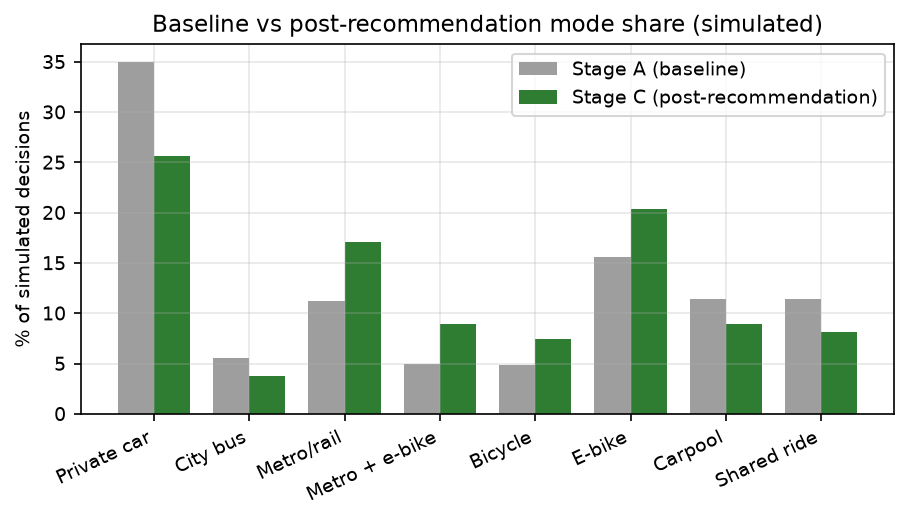
\includegraphics[width=0.92\textwidth]{fig_mode_share.png}
\caption{Baseline (Stage~A) versus post-recommendation (Stage~C) mode choice across 720 simulated
decisions.}
\label{fig:modeshare}
\end{figure}

\begin{table}[H]
\centering
\small
\caption{Behavioural and trade-off indicators, baseline versus recommendation (simulated
demonstration data).}
\label{tab:indicators}
\begin{tabular}{@{}lr@{}}
\toprule
\textbf{Indicator} & \textbf{Value}\\
\midrule
Baseline private-car share & 35.0\%\\
Post-recommendation private-car share & 25.6\%\\
Baseline sustainable-mode share & 65.0\%\\
Post-recommendation sustainable-mode share & 74.4\%\\
Recommendation acceptance rate (141 of 502 differing recommendations) & 28.1\%\\
Mode-shift rate (baseline car decisions moved off car) & 27.0\% (68 of 252)\\
Respondents with at least one shift & 48 (40.0\%)\\
Mean travel-time difference per trip (Stage C $-$ A) & $-0.15$ min\\
Mean cost difference per trip (Stage C $-$ A) & $-10.30$ rupees\\
Mean CO$_2$ difference per trip (Stage C $-$ A) & $-134.1$ g\\
\bottomrule
\end{tabular}
\end{table}

Recommendations were personalised through respondent-specific weights on time, cost and CO$_2$, but
the options in some scenarios were close enough that many respondents received the same
recommendation; recommended modes were E-bike (215), Metro/rail (198), Bicycle (136), Metro $+$ e-bike
(117), Carpool (34), City bus (15) and Private car (5). The rule recommended the private car in only 5
decisions, so reverse shifts toward the car were possible but rare.

\subsection{CO$_2$ Savings Analysis}
Using the emission model (Section~\ref{sec:emission}), baseline emissions averaged $717.0$~g CO$_2$ per
trip and post-recommendation emissions $582.8$~g, a mean saving of $134.1$~g per trip (95\% CI
$106.0$--$162.3$~g; $18.7\%$ reduction; paired $t(119) = -9.37$, $p < .001$; Cohen's $d_z = 0.35$).
Because the paired differences were not normally distributed (Shapiro--Wilk $p < .001$), the Wilcoxon
signed-rank test is preferred ($p < .001$) and leads to the same conclusion. Relative to an all-car
reference, mean per-trip emissions would be $1388.3$~g; baseline choices already avoid $671.3$~g and
post-recommendation choices $805.5$~g of that reference. Table~\ref{tab:co2} and Figure~\ref{fig:co2}
show results by scenario.

\begin{table}[H]
\centering
\small
\caption{Modelled CO$_2$ per trip by scenario (g; simulated demonstration data).}
\label{tab:co2}
\begin{tabular}{@{}lrrrrrr@{}}
\toprule
\textbf{Scenario} & \textbf{Distance} & \textbf{All-car ref.} & \textbf{Stage A mean} & \textbf{Stage C mean} & \textbf{Saving} & \textbf{Reduction}\\
\midrule
S1 & 3~km & 510 & 236.2 & 187.2 & 49.0 & 20.7\%\\
S2 & 6~km & 1020 & 443.9 & 334.2 & 109.7 & 24.7\%\\
S3 & 8~km & 1360 & 722.4 & 593.0 & 129.4 & 17.9\%\\
S4 & 12~km & 2040 & 1071.1 & 873.0 & 198.1 & 18.5\%\\
S5 & 15~km & 2550 & 1396.1 & 1150.9 & 245.2 & 17.6\%\\
S6 & 5~km & 850 & 432.2 & 358.8 & 73.4 & 17.0\%\\
All & --- & 1388 & 717.0 & 582.8 & 134.1 & 18.7\%\\
\bottomrule
\end{tabular}
\end{table}

\begin{figure}[H]
\centering
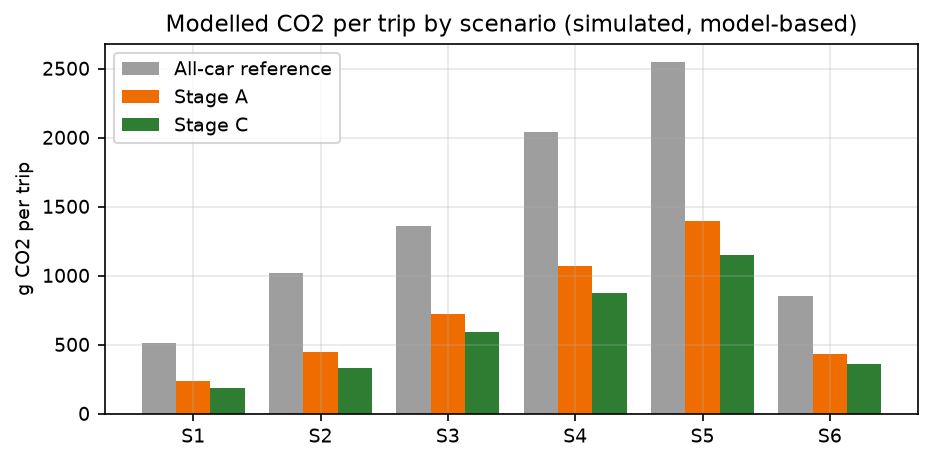
\includegraphics[width=0.92\textwidth]{fig_co2.png}
\caption{Modelled CO$_2$ per trip by scenario: all-car reference, simulated baseline (Stage~A) and
post-recommendation (Stage~C). Model-based illustration only.}
\label{fig:co2}
\end{figure}

\subsection{Illustrative Environmental Projection Based on Simulated Data}
This projection is \textbf{model-based and illustrative}; it is not observed environmental impact.
Assumptions: (i)~the six scenarios are equally weighted representative trips with a mean distance of
$8.2$~km (the mean of the six scenario distances; they are not each respondent's own commute);
(ii)~the mean simulated saving per trip of
$134.1$~g CO$_2$ persists; (iii)~a commuter makes 40 trips per month (20 commuting days $\times$ 2
trips); (iv)~an academic year of 9 months (360 trips); (v)~the emission factors of Table~\ref{tab:ef}
hold; (vi)~a hypothetical cohort of 1,000 commuters behaves like the simulated sample. Because
stated-choice responses commonly overstate real behaviour change, sensitivity rows apply $50\%$ and
$25\%$ of the simulated effect.

\begin{table}[H]
\centering
\small
\caption{Illustrative CO$_2$ projection from simulated data (model-based; not observed).}
\label{tab:projection}
\begin{tabular}{@{}lrrrr@{}}
\toprule
\textbf{Scenario} & \textbf{g/trip} & \textbf{kg/month} & \textbf{kg/year} & \textbf{tonnes/1{,}000 commuters/year}\\
\midrule
Baseline emissions (reference) & 717.0 & 28.7 & 258.1 & 258.1\\
100\% of simulated effect & 134.1 & 5.4 & 48.3 & 48.3\\
50\% of simulated effect & 67.1 & 2.7 & 24.1 & 24.1\\
25\% of simulated effect & 33.5 & 1.3 & 12.1 & 12.1\\
\bottomrule
\end{tabular}
\end{table}

Under the full simulated effect, savings would be $5.4$~kg CO$_2$ per commuter per month and
$48.3$~kg per academic year, or $48.3$ tonnes for 1{,}000 commuters. These figures depend entirely on
the simulation inputs and should not be quoted as expected real-world savings
(Figure~\ref{fig:projection}).

\begin{figure}[H]
\centering
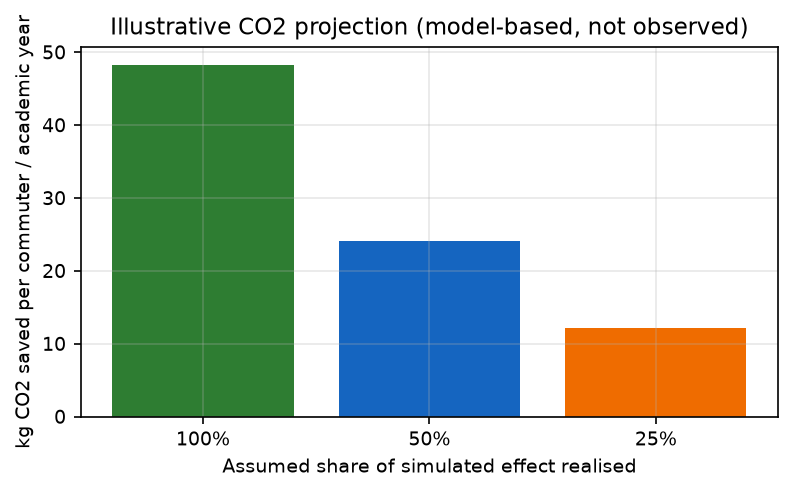
\includegraphics[width=0.7\textwidth]{fig_projection.png}
\caption{Illustrative CO$_2$ projection under assumed shares of the simulated effect
(model-based, not observed).}
\label{fig:projection}
\end{figure}

\subsection{Hypothesis Testing Summary}
Six hypotheses (seven tests) are summarised in Table~\ref{tab:hyp}. Results are demonstrations on
simulated data. Holm-adjusted $p$-values for the seven tests were: H1 $= .001$, H2 $= .785$, H3
$= .045$, H4 $= .017$, H5 $< .001$, H6a $< .001$, H6b $< .001$. H2 was not supported; all other
hypotheses were supported in the simulated data.

\begin{table}[H]
\centering
\small
\caption{Hypothesis testing summary (simulated demonstration data; $N = 120$).}
\label{tab:hyp}
\begin{tabular}{@{}p{3.9cm}p{1.9cm}p{2.5cm}rrp{2.2cm}@{}}
\toprule
\textbf{Hypothesis} & \textbf{Test} & \textbf{Simulated result} & \textbf{$p$} & \textbf{Holm $p$} & \textbf{Decision}\\
\midrule
H1: awareness $\rightarrow$ intention & Spearman $\rho$ & $\rho = .34$ & $<.001$ & .001 & Supported\\
H2: concern $\rightarrow$ shift count & Spearman $\rho$ & $\rho = .03$ & .785 & .785 & Not supported\\
H3: convenience $\rightarrow$ acceptance & Spearman $\rho$ & $\rho = .21$ & .023 & .045 & Supported\\
H4: private-vehicle users lower intention & Welch $t$ & $t = -2.83$ & .006 & .017 & Supported\\
H5: predictors jointly predict choice & Logistic LR & $\chi^2(6)=35.52$ & $<.001$ & $<.001$ & Supported\\
H6a: recommendation reduces car share & Wilcoxon & $W = 0.0$ & $<.001$ & $<.001$ & Supported\\
H6b: recommendation reduces CO$_2$/trip & Paired $t$ & $t = -9.37$ & $<.001$ & $<.001$ & Supported\\
\bottomrule
\end{tabular}
\end{table}

\section{Conceptual AI Framework: Eco-Friendly Daily Commute Helper}
\label{sec:framework}

\textbf{Status.} The framework is conceptual. It has not been implemented, deployed or empirically
validated. It retains the five-layer architecture of the original paper and connects it to the research
variables, the behavioural task and the evaluation metrics of this study. The conceptual chain is:
literature $\rightarrow$ research gap $\rightarrow$ research questions $\rightarrow$ variables
$\rightarrow$ instrument $\rightarrow$ statistical analysis $\rightarrow$ simulated findings
$\rightarrow$ behavioural and emission evaluation $\rightarrow$ AI framework $\rightarrow$ future
validation (Figure~\ref{fig:flow}).

The proposed helper has five layers (Figure~\ref{fig:five}), each tied to variables measured in the
proposed study.

\begin{figure}[H]
\centering
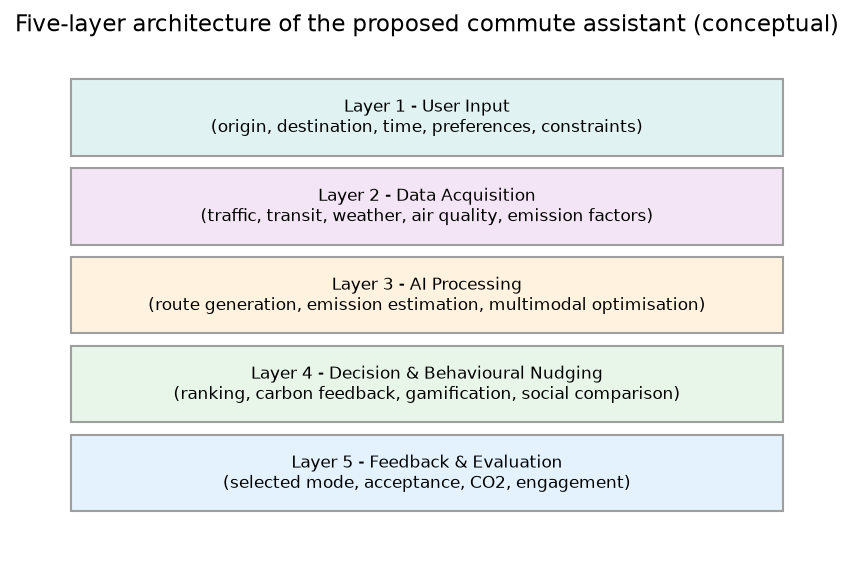
\includegraphics[width=0.82\textwidth]{fig_five_layer.png}
\caption{Five-layer architecture of the proposed AI-driven, behaviourally aware Eco-Friendly Daily
Commute Helper (conceptual).}
\label{fig:five}
\end{figure}

\subsection{Layer 1 --- User Input}
Collects origin, destination, departure time and user preferences (cost, time, comfort,
accessibility). In the research design, these correspond to \code{commute\_distance},
\code{commute\_days}, \code{current\_mode} and the decision-factor scores.

\subsection{Layer 2 --- Data Acquisition}
Gathers real-time traffic, public-transit schedules, weather and air-quality data, and emission factors
for each mode \citep{kashem2025,ouyang2025}. Emission factors would be regional and updated as grid and
fleet data change \citep{ndhlovu2025}. In the simulation, scenario times, costs and emission factors
are fixed design values.

\subsection{Layer 3 --- AI Processing}
Generates multimodal route options (walking, cycling, public transport, shared mobility, electric
vehicles), estimates emissions with Equations~\ref{eq:single}--\ref{eq:saved}, and predicts congestion
and energy use. This layer corresponds to the scenario option cards and the emission model of
Section~\ref{sec:emission}.

\subsection{Layer 4 --- Decision and Behavioural Nudging}
Ranks options on a multi-criteria basis (CO$_2$, travel time, cost, health benefit) with weights that
can be personalised, and reinforces low-emission choices through carbon feedback, gamified rewards and
social comparison. In the simulated Stage~B, the ranking used respondent-specific weights on time,
cost and CO$_2$ and displayed a recommendation card; gamification and social comparison were not
simulated.

\subsection{Layer 5 --- Feedback and Evaluation}
Logs the selected mode, measures impact (CO$_2$ saved, mode shift, engagement) and feeds results back
to personalise later recommendations. In the simulation, Stage~C choices and the derived indicators
play this role; no learning loop was simulated.

\subsection{Mapping Research Variables to System Components}
Table~\ref{tab:mapping} links research variables to system inputs, AI processes, behavioural
interventions and evaluation metrics. It describes design intent; it does not show that the framework
works.

\begin{table}[H]
\centering
\small
\caption{Mapping of research variables to system inputs, AI processes, behavioural interventions and
evaluation metrics.}
\label{tab:mapping}
\resizebox{\textwidth}{!}{%
\begin{tabular}{@{}p{2.9cm}p{3.2cm}p{3.0cm}p{3.1cm}p{2.3cm}@{}}
\toprule
\textbf{Research variable} & \textbf{System input (layer)} & \textbf{AI process (L3)} & \textbf{Behavioural intervention (L4)} & \textbf{Evaluation metric}\\
\midrule
\code{commute\_distance}; \code{current\_mode}; \code{commute\_days} & Origin, destination, time, usual mode (L1) & Multimodal route generation; distance-based option filtering & Mode-specific suggestions (e.g., bicycle on short trips) & Mode-shift rate; sustainable-mode share\\
\code{cost\_sensitivity}; \code{time\_sensitivity}; \code{convenience\_score}; comfort; safety; accessibility & Preference weights (L1) & Multi-criteria ranking with personalised weights & Rank and CO$_2$ display balancing time, cost, comfort & Cost and time difference; acceptance\\
\code{awareness\_score} & Optional profile baseline (L1) & Depth of explanation between options & CO$_2$ comparison cards & Awareness change (pre/post)\\
\code{concern\_score} & Optional profile baseline (L1) & Message framing around responsibility & Carbon feedback framed as environmental benefit & Mode-shift rate; concern change\\
\code{intention\_score} & Stated willingness by mode (L1) & Candidate-option filtering & Targeted prompts for intention change & Intention change; mode-shift rate\\
Traffic, transit, weather, air quality, emission factors & Real-time feeds and EF (L2) & Emission estimation ($E=d\times EF$); congestion prediction & Per-option CO$_2$ display & \code{baseline\_emission}; \code{recommended\_emission}; CO$_2$ saved\\
\code{acceptance\_score} (usefulness, trust, acceptance) & Interface feedback (L5) & Explanation of ranking & Transparency of recommendation card & Acceptance; continued use; trust\\
\code{engagement} & Usage logs (L5) & Personalised choice prompts & Gamified rewards; social comparison & User engagement; retention\\
\bottomrule
\end{tabular}}
\end{table}

\section{Evaluation Metrics}
\label{sec:metrics}

The original paper proposed five metrics. They are retained and extended with four metrics that capture
attitudes and trust. Table~\ref{tab:metrics} states what can be measured with the proposed survey and
what requires a real deployment or longitudinal follow-up. In this paper, only the metrics marked
``simulated'' were computed, and only on simulated data.

\begin{table}[H]
\centering
\small
\caption{Evaluation metrics and measurability.}
\label{tab:metrics}
\begin{tabular}{@{}p{3.2cm}p{6.2cm}p{2.6cm}p{2.4cm}@{}}
\toprule
\textbf{Metric} & \textbf{Definition} & \textbf{Measurable in proposed survey?} & \textbf{Status in this paper}\\
\midrule
Mode-shift rate & Share of baseline car decisions changed to a non-car option & Partly (stated choice) & Simulated\\
Sustainable-mode share & Share of decisions that are non-car & Yes & Simulated\\
Recommendation acceptance & Followed recommendations $\div$ differing recommendations & Partly (stated choice) & Simulated\\
CO$_2$ saved per trip & $E_{\text{car}}-E_{\text{selected}}$ (Section~\ref{sec:emission}) & Model-based only & Simulated\\
User engagement & Self-reported intention to continue use and check feedback & Yes (self-report) & Simulated\\
Awareness change & Pre/post change in \code{awareness\_score} & Requires pre/post design & Not computed\\
Concern change & Pre/post change in \code{concern\_score} & Requires pre/post design & Not computed\\
Trust in recommendations & Self-reported trust item (acc2) & Yes (self-report) & Simulated\\
Intention change & Pre/post change in \code{intention\_score} & Requires pre/post design & Not computed\\
\bottomrule
\end{tabular}
\end{table}

\section{Discussion}
\label{sec:discussion}

Four kinds of statement are kept apart below: published evidence (cited), simulated results (from the
demonstration dataset), the proposed framework, and projected outcomes (model-based). Interpretation
is the authors' reading.

\subsection{Interpretation of Literature}
The retained literature consistently identifies commuting as an addressable source of urban emissions
and the reduction of private-vehicle reliance as the recurring strategy \citep{comi2024,eslami2025}.
The benefit of each low-carbon option is conditional on infrastructure and urban design
\citep{marzolla2025}, on demographics, time, accessibility and affordability for electric
micromobility \citep{wu2025}, and on energy supply and uptake for electric vehicles
\citep{ndhlovu2025}. Digital tools are reported to support forecasting, route optimisation and
personalised advice \citep{kashem2025,ouyang2025}, while behavioural determinants influence whether
people act on information \citep{eslami2025}. \textit{Interpretation:} since benefits are conditional,
no single mode suits every commuter, so a measurement design should record both psycho-social
variables (awareness, concern, intention) and practical ones (cost, time, convenience), as this study
does.

\subsection{Findings from Simulated Data}
In the simulated data, awareness and intention were positively associated ($\rho = .34$), convenience
was associated with acceptance ($\rho = .21$), but concern was not significantly associated with mode
shift ($\rho = .03$) and private-vehicle users did report lower intention. In the logistic model, cost
sensitivity was a positive predictor and perceived convenience a negative predictor of a low-emission
majority; psycho-social predictors added little once practical factors were included. These patterns
were largely built into the generator (Section~\ref{sec:dataset}): the significant associations
illustrate how they would be reported, the null results how non-significant ones would be reported, and
none is evidence about real students. The baseline-versus-recommendation task produced a fall in
private-car share from $35.0\%$ to $25.6\%$ and a modelled $18.7\%$ reduction in CO$_2$ per trip, with
a negligible time penalty (mean $-0.15$~min) and a modelled cost saving; the direction follows from the
recommendation rule and the follow-probability model, so the magnitude depends on assumed inputs and
not on observed behaviour.

\subsection{Comparison with Previous Research}
The simulated results cannot be compared with previous research as independent evidence, because
agreement is by construction. Qualitatively, the design is consistent with the published emphasis on
practical conditions (time, affordability, accessibility) for micromobility use \citep{wu2025} and on
the combination of impact information with behavioural incentives \citep{eslami2025,niazi2024}.
Whether real students respond similarly to carbon-aware recommendations is an empirical question that
the retained sources do not answer. In particular, no retained source quantifies the effect of
personalised carbon feedback on commuting mode choice, so the magnitude seen in the simulation must
not be read as consistent or inconsistent with published effects.

\subsection{Implications for System Design}
For assistant design, the demonstration suggests that (i)~personalisation by cost and time weights
matters because practical factors dominated the baseline model; (ii)~options with little time penalty
and clear cost savings are the likeliest to be followed; and (iii)~the recommendation rule should be
transparent, because acceptance and trust were treated as attitudinal drivers of following
suggestions. These are design hypotheses for testing, not validated findings. The MaaS literature also
warns that digital integration alone does not guarantee environmental benefit unless low-carbon
options are prioritised \citep{an2025}, which supports including CO$_2$ explicitly in the ranking.

\subsection{Theoretical and Practical Implications}
The paper contributes a measurement-to-system mapping: each research construct has a defined place in
the five-layer architecture and a metric. Methodologically, it demonstrates reporting practice for
simulated data (labelling, disclosure of built-in structure, caution on agreement with prior work).
Practically, universities and developers can reuse the instrument and analysis plan for a genuine
pilot, and can use the data dictionary and variable mapping to log the same indicators in a real
system. The principal theoretical question left open is the relative contribution of psycho-social
variables and practical constraints to real recommendation uptake. Infrastructure and policy remain
preconditions: walking and cycling infrastructure, reliable public transport, real-time information
and integrated ticketing enable the behaviours that assistants seek to encourage
\citep{cui2024,marzolla2025}.

\section{Limitations}
\label{sec:limits}

The limitations below are substantial and should be read before any result is interpreted.
\begin{itemize}[leftmargin=*]
\item \textbf{Simulated rather than genuine data.} All numerical results come from a synthetic dataset
with built-in structure; they describe no real person and cannot be cited as findings.
\item \textbf{Proposed rather than completed sampling.} The survey, pilot, approvals and recruitment
have not taken place; the sample size of 150 is a plan.
\item \textbf{Convenience sampling (proposed)} would produce a non-probability sample with selection
bias.
\item \textbf{Single-institution context} limits generalisability to other universities, cities and
age groups.
\item \textbf{Self-report bias.} Awareness, concern and acceptance are self-reported and subject to
social-desirability bias.
\item \textbf{Scenario-based rather than real behaviour.} Stated choices in hypothetical trips may not
predict actual mode choice, and the within-subject design cannot rule out demand effects.
\item \textbf{Limited scenarios.} Six scenarios cannot represent all commuting conditions;
two-wheelers, a common commuting mode, are not modelled as a scenario option.
\item \textbf{Uncertain emission factors.} The factors are illustrative inputs; real values vary with
fleet, occupancy, fuel and grid.
\item \textbf{No real system deployment.} The commute assistant exists only as a design; no
recommendation engine was built or tested.
\item \textbf{No causal inference.} Cross-sectional associations and a within-subject hypothetical
comparison cannot establish causal effects of recommendations.
\item \textbf{Statistical limitations.} Several scales had modest reliability (time and convenience
below $.60$), the outcome group size gave about 7.2 events per predictor, trip-level tests ignore
clustering, and $p$-values reflect a generator, not a population.
\item \textbf{Uncertain projections.} Monthly and annual projections rest on equal-weight scenario
trips, a fixed trip count and an assumed persistence of effect.
\end{itemize}

\section{Conclusion}
The literature establishes that commuting is a significant, addressable source of urban emissions; that
low-carbon options are conditional on infrastructure, energy supply and user circumstances; that AI,
IoT and big-data tools can support forecasting, route optimisation and personalised advice; and that
behavioural mechanisms are determinants of success. The main gap is the absence of integrated,
personalised, behaviourally aware commute assistants and of measurable designs for evaluating them.

The quantitative methodology was designed to investigate sustainable-commuting awareness, concern,
intention and mode choice, and the response to personalised recommendations. The paper specifies a
cross-sectional, scenario-based design with research questions, hypotheses, variables, a seven-section
instrument, a data dictionary, an emission model and a statistical analysis plan, all mapped to one
another.

The simulated analysis demonstrated that the analysis plan runs end to end on a clearly labelled
synthetic dataset of 120 respondents: descriptive statistics, reliability, normality checks,
correlation, group comparisons, logistic regression, a conditional mode-choice model, a
baseline-versus-recommendation comparison and a CO$_2$ projection. Of the six hypotheses, those built
into the generator were detected and the others were not, which illustrates both significant and null
reporting. In the simulated demonstration scenario, the model projected an illustrative $18.7\%$
reduction in CO$_2$ per trip and an illustrative $5.4$~kg saving per commuter per month under stated
assumptions. These are demonstrations of the procedure and projections from a model; they are not
evidence about real commuters or observed environmental effects.

The conceptual framework contributes a five-layer architecture with an explicit mapping from research
variables to system inputs, AI processes, behavioural interventions and evaluation metrics. What
remains unvalidated is everything empirical: real awareness, concern and intention levels; real
recommendation acceptance and mode shift; real CO$_2$ savings; and the performance of any implemented
assistant. These require genuine data collection and pilot deployment.

\section{Recommendations}
\subsection{A. Supported by Existing Literature}
\begin{enumerate}[leftmargin=*]
\item Design commute assistants around multimodal options (public transport, active travel,
micromobility, shared mobility and electric vehicles) rather than a single mode, because integrated
ecosystems are under-researched and ease of multimodal planning is associated with acceptance
\citep{kashem2025,smith2023}.
\item Base emission estimates on regional, regularly updated emission factors, because the benefit of
electric options depends on the electricity source \citep{ndhlovu2025}.
\item Orient MaaS and similar platforms explicitly towards low-carbon options, since adoption alone
does not guarantee environmental benefit \citep{an2025}.
\item Combine environmental-impact information with behavioural mechanisms such as incentives rather
than relying on information alone \citep{eslami2025,niazi2024}.
\item Pair digital tools with supportive infrastructure and policy, including walking and cycling
infrastructure, reliable public transport, real-time transit information and integrated ticketing
\citep{cui2024,marzolla2025}.
\item Adopt interdisciplinary approaches that bring together urban planning, behavioural science and
digital technology \citep{eslami2025}.
\end{enumerate}

\subsection{B. Requiring Future Empirical Validation}
\begin{enumerate}[leftmargin=*]
\item Which nudging mechanisms (carbon feedback, gamified rewards, social comparison) are most
effective, and how to weight CO$_2$, time, cost and health in the ranking, should be established by
pilot evaluation, not assumed.
\item Claims about mode shift, recommendation acceptance and emission savings should be made only
after the metrics in Section~\ref{sec:metrics} have been measured with genuine data.
\item Whether psycho-social variables or practical constraints better predict real recommendation
uptake should be tested with a genuine survey and observed behaviour.
\item The instrument's reliability and validity, in particular the short three-item scales, should be
confirmed in a pilot before the main survey.
\end{enumerate}

\section{Future Scope}
\begin{enumerate}[leftmargin=*]
\item Real survey deployment at Chandigarh University after piloting and approvals, replacing the
simulated dataset.
\item Larger samples (beyond $n \approx 150$) and multi-university samples to improve
generalisability.
\item A pilot of the commute assistant with a small group of volunteers.
\item Integration of real mobility data and real transit data (schedules, delays, fares).
\item Validated regional emission factors, including two-wheelers and local grid mix.
\item A/B testing of recommendation designs (with and without CO$_2$ feedback, gamification, social
comparison).
\item Longitudinal behavioural tracking of observed mode choice and engagement.
\item Pre-test/post-test intervention designs measuring changes in awareness and intention.
\item Real-world CO$_2$ measurement or logged-trip emission estimation.
\item Machine-learning optimisation and personalised recommendation algorithms trained on genuine
data.
\item Comparison of recommendation algorithms (e.g., rule-based ranking versus learned policies).
\item Integration with MaaS platforms, designed to favour low-carbon options.
\item A more exhaustive systematic literature review to reduce selection bias inherent in the
original narrative review.
\end{enumerate}

\begin{thebibliography}{99}
\setlength{\itemsep}{0.2em}
\bibitem[An \& Shen(2025)]{an2025} An, C., \& Shen, J. (2025). Assessing the impact of
Mobility-as-a-Service (MaaS) on sustainable urban travel behaviors: A systematic literature review.
\emph{Frontiers in Sustainable Cities, 7}, 1645488.
\bibitem[Bamberg \& M\"oser(2007)]{bamberg2007} Bamberg, S., \& M\"oser, G. (2007). Twenty years
after Hines, Hungerford, and Tomera: A new meta-analysis of psycho-social determinants of
pro-environmental behaviour. \emph{Journal of Environmental Psychology, 27}(1), 14--25.
\bibitem[Cats et al.(2017)]{cats2017} Cats, O., Susilo, Y. O., \& Reimal, T. (2017). The prospects of
fare-free public transport: Evidence from Tallinn. \emph{Transportation, 44}(5), 1083--1104.
\bibitem[Collazos et al.(2024)]{collazos2024} Collazos, J. S. G., Ardila, L. M. C., \& Cardona, C. J.
F. (2024). Energy transition in sustainable transport: Concepts, policies, and methodologies.
\emph{Environmental Science and Pollution Research, 31}(49), 58669--58686.
\bibitem[Comi \& Polimeni(2024)]{comi2024} Comi, A., \& Polimeni, A. (2024). Assessing potential
sustainability benefits of micromobility: A data-driven approach. \emph{European Transport Research
Review, 16}, 19.
\bibitem[Creutzig et al.(2015)]{creutzig2015} Creutzig, F., Jochem, P., Edelenbosch, O. Y., Mattauch,
L., Vuuren, D. P. V., McCollum, D., \& Minx, J. (2015). Transport: A roadblock to climate change
mitigation? \emph{Science, 350}(6263), 911--912.
\bibitem[Cui \& Zhang(2024)]{cui2024} Cui, C., \& Zhang, Y. (2024). Integration of shared
micromobility into public transit: A systematic literature review with grey literature.
\emph{Sustainability, 16}(9), 3557.
\bibitem[Eslami(2025)]{eslami2025} Eslami, E. (2025). \emph{Carbon-negative commuting: Integrating
urban design, behavior, and technology for climate-positive mobility} (arXiv preprint
arXiv:2509.21440).
\bibitem[Garus et al.(2024)]{garus2024} Garus, A., Mourtzouchou, A., Suarez, J., Fontaras, G., \&
Ciuffo, B. (2024). Exploring sustainable urban transportation: Insights from shared mobility services
and their environmental impact. \emph{Smart Cities, 7}(3), 1199--1220.
\bibitem[Hensher(2024)]{hensher2024} Hensher, D. A. (2024). The future of mobility as a service.
\emph{Transportation Planning and Technology, 47}(5), 624--627.
\bibitem[Kashem et al.(2025)]{kashem2025} Kashem, M. A., Shamsuddoha, M., \& Nasir, T. (2025).
Digitalization in sustainable transportation operations: A systematic review of AI, IoT, and
blockchain applications for future mobility. \emph{Future Transportation, 5}(4), 157.
\bibitem[L\"attman \& Otsuka(2024)]{lattman2024} L\"attman, K., \& Otsuka, N. (2024). Sustainable
development of urban mobility through active travel and public transport. \emph{Sustainability,
16}(2), 534.
\bibitem[Liu et al.(2025)]{liu2025} Liu, Y., Zhou, D., \& Wu, C. (2025). Strategies for sustainable
road transport: Technological innovation and organizational management through AI.
\emph{Transportation Research Part D: Transport and Environment, 141}, 104651.
\bibitem[Marzolla et al.(2025)]{marzolla2025} Marzolla, F., Bruno, M., Melo, H. P., \& Loreto, V.
(2025). \emph{Proximity-based cities emit less mobility-driven CO$_2$} (arXiv preprint
arXiv:2510.00094).
\bibitem[Mogire(2025)]{mogire2025} Mogire, E. (2025). \emph{Light electric vehicles and sustainable
urban transport: A bibliometric review}.
\bibitem[Ndhlovu et al.(2025)]{ndhlovu2025} Ndhlovu, E., Mhlanga, D., \& Duri, B. (2025).
Decarbonising urban transport: An overview of electric vehicles, public transport, and sustainable
infrastructure in achieving net-zero emissions. \emph{Discover Global Society, 3}(1), 53.
\bibitem[Niazi et al.(2024)]{niazi2024} Niazi, M. U. B., Cho, J. H., Dahleh, M. A., Dong, R., \& Wu,
C. (2024). Incentive design for eco-driving in urban transportation networks. In \emph{2024 European
Control Conference (ECC)} (pp. 986--991). IEEE.
\bibitem[Nisa et al.(2025)]{nisa2025} Nisa, C., Gu, M., \& B\'elanger, J. J. (2025). Eliciting
attachment security with social norm messages is linked to reduced energy consumption in extreme heat
in the United Arab Emirates. \emph{Communications Earth \& Environment, 6}(1), 315.
\bibitem[Ouyang et al.(2025)]{ouyang2025} Ouyang, S., Zhao, P., \& Gong, Z. (2025). A review of
transport carbon emissions: Insights from artificial intelligence and big data. \emph{Journal of
Cleaner Production, 532}, 146906.
\bibitem[Shaheen \& Cohen(2018)]{shaheen2018} Shaheen, S., \& Cohen, A. (2018). Shared mobility
policies for California. \emph{ITS Berkeley Policy Briefs, 2018}(03).
\bibitem[Smith et al.(2023)]{smith2023} Smith, G., Hensher, D. A., Ho, C., \& Balbontin, C. (2023).
Mobility-as-a-Service users: Insights from a trial in Sydney. \emph{European Transport Research
Review, 15}(1), 40.
\bibitem[Sunio(2018)]{sunio2018} Sunio, V. C. (2018). \emph{Mobility behavior change support system
for sustainable campus commuting}.
\bibitem[Wu et al.(2025)]{wu2025} Wu, Y., Yildirimoglu, M., \& Zheng, Z. (2025). \emph{Evaluating
electric micro-mobility related mode choice stated preferences: A latent class choice approach}
(arXiv preprint arXiv:2504.01237).
\end{thebibliography}

\noindent\textit{Note.} Reference details are those of the original paper, preserved without
addition. Entries for which the source material gave no venue (Mogire, 2025; Sunio, 2018) are left as
given. All references listed here are cited in the text.

\appendix

\section{Appendix A --- Full Questionnaire}
\label{app:questionnaire}

\textbf{Participant questionnaire (proposed; not yet administered).} \textit{Informed consent:} You are
invited to take part in a research study on sustainable commuting among university students.
Participation is voluntary and you may withdraw at any stage. No names, passwords or financial details
are collected. Responses are anonymous and used only for academic research. By proceeding you confirm
that you are 18 or older and agree to participate.

\subsection*{Section A --- Commuting profile}
A1 Age (years). A2 Gender (Male / Female / Other-prefer not to say). A3 Year of study (1--4).
A4 Programme (CSE / Other engineering / Management-Commerce / Sciences-Other). A5 One-way distance to
campus ($<$2~km / 2--5~km / 5--10~km / $>$10~km). A6 Main current mode (Private car / Two-wheeler /
Bus / Walking-Cycling / Carpool-Shared ride). A7 Days per week you travel to campus (3--6).

\subsection*{Section B --- Sustainable mobility awareness (1 = strongly disagree \dots\ 5 = strongly agree)}
B1. I know which commuting options (e.g., walking, cycling, bus, metro, carpool, e-bike) produce lower
CO$_2$ emissions than a private car. B2. I understand that private-car commuting contributes
substantially to urban greenhouse-gas emissions. B3. I am aware that public transport can emit less
CO$_2$ per passenger-km than a solo car trip. B4. I know that walking and cycling produce almost no
tailpipe emissions and bring health benefits. B5. I am aware that carpooling or ride-sharing can reduce
the number of vehicles on the road. B6. I am aware that shared e-bikes and e-scooters can replace short
car trips. B7. I understand that the environmental benefit of electric vehicles depends on how the
electricity is generated. B8. I know of mobile apps or digital tools that show multimodal routes or
travel emissions. B9. I can roughly judge which of two travel options has the lower CO$_2$ impact.
B10. Attention check (unscored): For quality control, please select ``Agree'' (4) for this item.

\subsection*{Section C --- Environmental concern and attitudes (same 1--5 scale)}
C1. I am concerned about air pollution caused by road traffic in my city. C2. I am concerned about the
effect of transport emissions on climate change. C3. I feel a personal responsibility to reduce the
emissions caused by my daily travel. C4. I feel uncomfortable choosing a high-emission option when a
cleaner one is available. C5. I believe that individual commuting choices make a difference to the
environment. C6. I think universities should encourage low-emission commuting. C7. Reducing my travel
emissions is important to me even if it takes slightly longer.

\subsection*{Section D --- Commuting decision factors (same 1--5 scale)}
D1. Low travel cost is a major factor in my choice of commute mode. (cost1) D2. I would switch to a
cheaper option even if it were less comfortable. (cost2) D3. I check the cost of alternatives before
travelling. (cost3) D4. Short travel time is a major factor in my choice. (time1) D5. I would pay more
to reach campus faster. (time2) D6. Unexpected delays strongly affect my choice of mode. (time3)
D7. I prefer a door-to-door option that needs no transfers. (conv1) D8. Flexibility to leave at any
time is important to me. (conv2) D9. Ease of planning and boarding (no long waits, no complicated
tickets) is important to me. (conv3) D10. Comfort (seating, temperature, protection from weather) is
important to me. (comfort) D11. Personal safety, including at night, is important to me. (safety)
D12. Having a stop, station, bike or ride service close to my home and to campus is important to me.
(access)

\subsection*{Section E --- Sustainable travel intention}
Over the next semester, how willing are you to use the following for your commute?
(1 = very unwilling \dots\ 5 = very willing). E1 Walking. E2 Cycling. E3 Public transport
(bus/metro/rail). E4 Carpooling. E5 Shared mobility (e.g., shared e-scooter or pooled ride).
E6 E-bike or e-scooter. E7 Electric vehicle (own or shared).

\subsection*{Section F --- Scenario-based commute choice (Stage A)}
For each of six trips (Appendix~\ref{app:scenarios}) choose the option you would most likely take. Cards
show time, cost, comfort and convenience.

\subsection*{Section G --- Recommendation and assistant acceptance}
G1: For each scenario, a personalised recommendation card (time, cost, CO$_2$, convenience,
environmental benefit) is shown; choose again (Stage C). G2: Rate agreement (1--5) with: G2-1. Such an
assistant would be useful for planning my commute. (acc1) G2-2. I would trust the time, cost and CO$_2$
information it shows. (acc2) G2-3. I would accept its recommended option when it is reasonable. (acc3)
G2-4. I would be willing to follow its suggestions even if my usual mode is different. (acc4) G2-5.
Seeing the CO$_2$ impact of each option would add value to my decisions. (acc5) G2-6. I would continue
to use such an assistant over the semester. (acc6) G2-7. I would regularly check CO$_2$ feedback or my
carbon-saving summary. (acc7)

\section{Appendix B --- Scenario-Based Commute Choice Items}
\label{app:scenarios}

Scenario values are illustrative design values and do not describe real services. Comfort and
convenience are 1--5 ratings shown to respondents as star ratings. CO$_2$ (g, from
Equations~\ref{eq:single}--\ref{eq:multi}) is displayed only in Stage~B and is withheld in Stage~A.

\footnotesize
\begin{longtable}{@{}p{3.4cm}p{2.2cm}rrrrr@{}}
\caption{Scenario option cards (time in minutes; cost in rupees).}
\label{tab:B1}\\
\toprule
\textbf{Scenario} & \textbf{Option} & \textbf{Time} & \textbf{Cost} & \textbf{Comfort} & \textbf{Conv.} & \textbf{CO$_2$ (g)}\\
\midrule
\endfirsthead
\toprule
\textbf{Scenario} & \textbf{Option} & \textbf{Time} & \textbf{Cost} & \textbf{Comfort} & \textbf{Conv.} & \textbf{CO$_2$ (g)}\\
\midrule
\endhead
\bottomrule
\endlastfoot
S1: Short campus-area trip, fair weather, off-peak (3~km) & Private car & 12 & 40 & 4 & 5 & 510\\
 & City bus & 20 & 10 & 2 & 3 & 210\\
 & Bicycle & 15 & 0 & 2 & 3 & 0\\
 & E-bike & 11 & 25 & 3 & 4 & 60\\
 & Shared ride & 13 & 30 & 3 & 4 & 180\\
\midrule
S2: Peak-hour trip, congested corridor (6~km) & Private car & 25 & 85 & 4 & 5 & 1020\\
 & City bus & 35 & 15 & 2 & 3 & 420\\
 & Bicycle & 28 & 0 & 2 & 3 & 0\\
 & Carpool & 27 & 30 & 3 & 3 & 342\\
 & E-bike & 19 & 45 & 3 & 4 & 120\\
\midrule
S3: Hot, humid day, medium distance (8~km) & Private car & 22 & 110 & 4 & 5 & 1360\\
 & City bus & 38 & 12 & 2 & 3 & 560\\
 & Metro/rail & 28 & 25 & 4 & 4 & 240\\
 & Carpool & 25 & 40 & 3 & 3 & 456\\
 & Shared ride & 30 & 70 & 3 & 4 & 480\\
\midrule
S4: Rainy day, longer distance (12~km) & Private car & 35 & 170 & 4 & 5 & 2040\\
 & City bus & 50 & 15 & 2 & 3 & 840\\
 & Metro/rail & 38 & 40 & 4 & 4 & 360\\
 & Carpool & 38 & 60 & 3 & 3 & 684\\
 & Shared ride & 40 & 110 & 3 & 4 & 720\\
\midrule
S5: Long trip with first/last-mile leg (15~km) & Private car & 40 & 210 & 4 & 5 & 2550\\
 & Metro $+$ e-bike & 45 & 45 & 4 & 3 & 420\\
 & City bus & 60 & 30 & 2 & 3 & 1050\\
 & Carpool & 44 & 75 & 3 & 3 & 855\\
 & Shared ride & 48 & 140 & 3 & 4 & 900\\
\midrule
S6: Evening return trip, personal-safety concern (5~km) & Private car & 18 & 70 & 4 & 5 & 850\\
 & City bus & 30 & 15 & 2 & 3 & 350\\
 & Carpool & 20 & 30 & 3 & 3 & 285\\
 & Shared ride & 22 & 60 & 3 & 4 & 300\\
 & E-bike & 15 & 35 & 3 & 4 & 100\\
\end{longtable}

\section{Appendix C --- Variable Coding Scheme}
\label{app:coding}

\begin{table}[H]
\centering
\small
\caption{Coding and scoring rules.}
\label{tab:C1}
\begin{tabular}{@{}p{3.4cm}p{11.5cm}@{}}
\toprule
\textbf{Item} & \textbf{Rule}\\
\midrule
Likert items & $1 =$ strongly disagree / very unwilling \dots\ $5 =$ strongly agree / very willing; no reverse-keyed items\\
Scale scores & Arithmetic mean of items (awareness: aw1--9; concern: ec1--7; cost: cost1--3; time: time1--3; convenience: conv1--3; intention: int1--7; acceptance: acc1--acc6)\\
\code{engagement} & Mean of acc6 and acc7\\
Mode codes & C private car; B city bus; M metro/rail; Y bicycle; E e-bike; P carpool; S shared ride; X metro $+$ e-bike\\
Sustainable choice & Any code other than C\\
\code{low\_emission\_majority} & 1 if at least 4 of 6 Stage~A choices are not C\\
Recommendation followed & Stage C $=$ recommendation and recommendation $\neq$ Stage A\\
Acceptance rate & Followed $\div$ number of decisions where recommendation $\neq$ Stage A\\
Mode shift & Stage A $=$ C and Stage C $\neq$ C; \code{shift\_count} $=$ number of such scenarios; indicator $=1$ if count $\geq 1$\\
Emission per decision & $E = d \times EF_m$ (Section~\ref{sec:emission}); \code{baseline\_emission} $=$ mean over six Stage~A choices; \code{recommended\_emission} $=$ mean over six Stage~C choices\\
Attention check / exclusion & Fail attention item, speeding ($<$ one-third median time) or straight-lining $\rightarrow$ excluded (proposed rule)\\
\bottomrule
\end{tabular}
\end{table}

\section{Appendix D --- Item-Level Data Dictionary}
\label{app:datadict}

Item-level variables and their meanings are listed in Table~\ref{tab:datadict}
(Section~\ref{sec:datadict}) and in the full questionnaire (Appendix~\ref{app:questionnaire}). Each
item is an integer from 1 to 5. Items map to constructs as follows: aw1--aw9 $\rightarrow$
\code{awareness\_score}; ec1--ec7 $\rightarrow$ \code{concern\_score}; cost1--cost3 $\rightarrow$
\code{cost\_sensitivity}; time1--time3 $\rightarrow$ \code{time\_sensitivity}; conv1--conv3
$\rightarrow$ \code{convenience\_score}; int1--int7 $\rightarrow$ \code{intention\_score}; acc1--acc6
$\rightarrow$ \code{acceptance\_score}; acc6--acc7 $\rightarrow$ \code{engagement}. The complete
simulated dataset, including all item-level values, accompanies this paper as
\code{simulated\_dataset.csv}.

\section{Appendix E --- Simulated Dataset}
\label{app:dataset}

The full synthetic dataset of $N = 120$ respondents is provided as a machine-readable file
(\code{simulated\_dataset.csv}) generated by \code{simulation\_analysis.py} with fixed seed
\code{20251006}. Table~\ref{tab:extract} reproduces a representative extract of 20 respondents. The
extract is sufficient to show the structure; the full file contains every item and every derived
variable described in Section~\ref{sec:datadict}. \textbf{These are simulated values: the respondents
are fictional and no real person provided any value.}

\begin{table}[H]
\centering
\small
\caption{Representative extract of the simulated demonstration dataset (first 20 of 120 fictional
respondents).}
\label{tab:extract}
\begin{tabular}{@{}llllrrrrr@{}}
\toprule
\textbf{ID} & \textbf{Age} & \textbf{G.} & \textbf{Dist.} & \textbf{Current mode} & \textbf{Aware.} & \textbf{Intent.} & \textbf{Accept.} & \textbf{CO$_2$ saved (g)}\\
\midrule
R001 & 21 & F & $<$2 & Carpool/Shared & 4.44 & 4.71 & 4.33 & 57\\
R002 & 20 & F & $<$2 & Walking/Cycling & 4.56 & 3.86 & 3.83 & 0\\
R003 & 18 & F & 2--5 & Bus & 3.89 & 3.14 & 4.33 & 187\\
R004 & 19 & M & $>$10 & Bus & 3.78 & 3.14 & 4.00 & 74\\
R005 & 21 & M & $>$10 & Carpool/Shared & 3.33 & 3.57 & 3.67 & 150\\
R006 & 19 & M & 5--10 & Private car & 1.89 & 4.00 & 3.17 & 320\\
R007 & 19 & F & $>$10 & Bus & 4.00 & 2.86 & 3.83 & 105\\
R008 & 20 & F & $>$10 & Carpool/Shared & 2.56 & 3.00 & 2.83 & 60\\
R009 & 18 & M & 2--5 & Walking/Cycling & 3.11 & 3.43 & 3.67 & 105\\
R010 & 21 & M & $>$10 & Bus & 3.67 & 4.00 & 4.17 & 53\\
R011 & 22 & F & 5--10 & Private car & 3.11 & 4.29 & 1.83 & 0\\
R012 & 20 & F & 5--10 & Bus & 2.67 & 2.29 & 3.50 & 0\\
R013 & 21 & F & 5--10 & Carpool/Shared & 2.22 & 3.00 & 4.33 & 159\\
R014 & 20 & M & $<$2 & Private car & 4.22 & 3.86 & 5.00 & 537\\
R015 & 20 & M & 2--5 & Bus & 3.11 & 4.14 & 4.17 & 266\\
R016 & 18 & M & $<$2 & Bus & 4.78 & 4.71 & 3.67 & 54\\
R017 & 21 & M & 2--5 & Private car & 3.00 & 3.43 & 3.50 & 0\\
R018 & 21 & M & $>$10 & Two-wheeler & 4.67 & 4.43 & 3.33 & 99\\
R019 & 20 & M & $<$2 & Walking/Cycling & 4.44 & 4.00 & 3.33 & 85\\
R020 & 19 & M & $>$10 & Carpool/Shared & 3.11 & 4.14 & 4.00 & 592\\
\bottomrule
\end{tabular}
\end{table}

\noindent\textit{Generation summary.} Demographics and commute-distance categories were drawn from the
assumed distributions in Section~\ref{sec:dataset}; current mode was drawn conditional on distance;
correlated latent traits were transformed into Likert items with added noise; Stage~A choices came from
a random-utility model; recommendations were produced by a personalised weighted ranking; and Stage~C
choices followed the recommendation with a probability that increased with acceptance. All steps used
the single seed \code{20251006}, so the dataset and every statistic in Section~\ref{sec:results} are
exactly reproducible.

\section{Appendix F --- Statistical Analysis Output Tables}
\label{app:stats}

The complete machine-readable statistical output is provided as \code{analysis\_output.json}. It
contains: descriptives (mean, $SD$, median, min, max, skewness, kurtosis, Shapiro--Wilk) for every
composite; Cronbach's alpha for every multi-item scale; the full Spearman correlation matrix; the
group-comparison statistics (Welch $t$ with degrees of freedom and Cohen's $d$; Mann--Whitney $U$ with
rank-biserial $r$; Kruskal--Wallis $H$); the binary logistic-regression coefficients, standard errors,
$p$-values, odds ratios and confidence intervals; the conditional-logit attribute coefficients; the
baseline-versus-recommendation mode counts and indicators; the per-scenario CO$_2$ means; the
projection figures; and the hypothesis-testing summary with Holm-adjusted $p$-values. The key values
are reproduced in Tables~\ref{tab:desc}--\ref{tab:hyp} of the main text.

\section{Appendix G --- Five-Layer System Architecture}
\label{app:arch}

The five layers are summarised in Table~\ref{tab:arch}. Each layer is conceptual and has not been
implemented.

\begin{table}[H]
\centering
\small
\caption{Five-layer architecture (conceptual) and its research linkage.}
\label{tab:arch}
\begin{tabular}{@{}p{2.2cm}p{5.2cm}p{7.4cm}@{}}
\toprule
\textbf{Layer} & \textbf{Function} & \textbf{Research linkage}\\
\midrule
1 --- User input & Origin, destination, time, preferences, constraints & \code{commute\_distance}, \code{current\_mode}, \code{commute\_days}, decision-factor scores\\
2 --- Data acquisition & Traffic, transit, weather, air quality, emission factors & Layer~2 feeds the emission model (Section~\ref{sec:emission}); factors would be regional\\
3 --- AI processing & Route generation, emission estimation, multimodal optimisation, prediction & Scenario option cards; Equations~\ref{eq:single}--\ref{eq:saved}\\
4 --- Decision and nudging & Multi-criteria ranking, carbon feedback, gamification, social comparison & Stage~B recommendation card; personalised weights on time, cost, CO$_2$\\
5 --- Feedback and evaluation & Log selected mode, measure impact, feed back to personalise & Stage~C choices; mode-shift, acceptance, CO$_2$ and engagement metrics\\
\bottomrule
\end{tabular}
\end{table}

\section{Appendix H --- Proposed Evaluation Metrics}
\label{app:metrics}

The proposed evaluation metrics, their definitions and their measurability are given in
Table~\ref{tab:metrics}. In the present paper only the metrics marked ``Simulated'' were computed, and
only on the simulated dataset. The remaining metrics (awareness, concern and intention change) require
a genuine pre/post design and were not computed.

\end{document}
